\chapter{Úvod}

Cieľom tejto bakalárskej práce je návrh architektúry a následná implementácia aplikácie určenej na extrakciu dát z webových stránok. V dnešnej dobe je pojem extrakcia dát používaný stále častejšie, a to práve v spojitosti s webovými technológiami a webom samotným. Je to tak pravdepodobne preto, že sa internet ako taký, a hlavne jeho obsah v podobe webových stránok, neustále rozširuje. Objem dát, ktorý sa na webe nachádza, sa zväčšuje neúprosnou rýchlosťou, a preto je zber údajov z rôznych webových stránok stále zložitejší. A to nielen čo sa zložitosti štruktúry webu týka, ale vzhľadom na veľký počet webov sa zvyšuje aj časová náročnosť analýzy a následnej extrakcie dát. Takejto extrakcii sa hovorí web scraping. Web scraping môže prebiehať aj manuálne, kde ho vykonáva určená osoba, avšak v dnešnej dobe je už táto procedúra automatizovaná.

Práve pre spomínanú expanziu internetu sa tejto téme venuje čoraz viac spoločností, so snahou uľahčiť prístup k web scrapingu pre každodenných používateľov. Pre neustály vývoj webu je avšak nutné vyvíjať aj aplikácie, ktoré sú na extrakciu určené. 

Pri rozlišovaní takýchto aplikácií sa berie na vedomie hlavne požadovaný vstupný formát a jeho zložitosť, výstupný formát a jeho využiteľnosť v praxi a v neposlednom rade rýchlosť aplikácie z pohľadu extrakcie dát. 

Táto práca je zameraná hlavne na časť týkajúcu sa požadovaného vstupu aplikácie. Hlavným cieľom aplikácie je umožniť vyjadrenie požadovaných vstupných parametrov tak, aby neboli závislé na štruktúre webovej stránky, ale na jej obsahu. Na dosiahnutie tohto cieľa je potrebné vstupné údaje správne definovať, pretože práve na týchto vstupných údajoch bude závislá úspešnosť následnej extrakcie dát. Cieľom je teda možnosť definovať vstupné pravidlá jednoducho a v závislosti na požadovanom výstupe. Nebude ďalej potrebné poznať štruktúru webovej stránky. Ideálne vstupné pravidlá by mali pozostávať zo zoznamu adries webových stránok a štruktúre požadovaných údajov. Aplikácia sa následne pozerá na každú stránku zvlášť a určí výsledné údaje na základe poskytnutých relevantných informácií. Týmto spôsobom je možné definovať jeden vstup raz a použiť ho na viaceré webové dokumenty bez nutnosti ďalšieho zásahu. Zároveň by malo byť umožnené extrahovať akékoľvek údaje z akejkoľvek stránky, bez nutnosti analýzy danej webovej stránky alebo poznania jej vnútornej štruktúry. Vstupné a výstupné údaje budú taktiež používateľsky prívetivé tak, aby nebol kladený dôraz na skúsenosti s programovaním a programovacími jazykmi.

\newpage

Práca je rozdelená do 7 kapitol, z ktorých každá predstavuje časť vývoja finálnej aplikácie. Od predstavenia aktuálnej problematiky a technológií, ktoré sú v súčastnosti dostupné až po finálne testovanie aplikácie a zhodnotenie výsledkov.

\bigskip

Prvá časť práce sa v kapitole \ref{aktualny_pristup} zaoberá aktuálnym prístupom k problematike, ako sa web scraping využíva v súčasnosti, aké sú štandardy a dostupné technológie a porovnanie týchto prístupov z hľadiska využiteľnosti.

V druhej časti tejto práce sú v kapitole \ref{Technologie} popísané technológie, ktoré je treba brať \mbox{v úvahu} pri návrhu, tvorbe a analýze aplikácie určenej na extrakciu dát. Jedná sa hlavne o~technológie, ktoré sa stali základným kameňom navrhnutej aplikácie a na základe ktorých aplikácia stavia.

Kapitola \ref{Navrh} sa zameriava na analýzu a návrh architektúry aplikácie. Je založená na analýze špecifikácie, požiadaviek aplikácie a popisuje postup návrhu.

V \ref{implementacia}. kapitole sú popísané jednotlivé detaily implementácie riešenia a hlavná logika aplikácie.

\ref{testing}. kapitola sa následne venuje testovaniu aplikácie za pomoci niekoľkých testovacích sád, následnej analýze a vyhodnotení výsledkov, ktoré aplikácia dosiahla.


\chapter{Aktuálny prístup k problematike Web Scrapingu}
\label{aktualny_pristup}

V tejto kapitole sú uvedené a popísané aktuálne prístupy, ktoré sa používajú na extrakciu dát z webových dokumentov. Takáto extrakcia môže prebiehať online alebo offline, v~závislosti na tom aké dáta a za akým cieľom ich chceme extrahovať.

Web scrapingu sa v súčasnosti venuje stále viac a viac spoločností, a preto nieje prekvapením, že sa rozširujú nielen možnosti web scrapingových aplikácií, ale aj prístup takýchto aplikácií k priamej extrakcii dát.

Zároveň sa rozširuje pole pôsobnosti a možnosti využitia takto extrahovaných dát. Preto je táto kapitola určená hlavne rozboru týchto metód. Poznatky získané z tohto rozboru zároveň pomôžu určiť smer, ktorým sa návrh a vývoj aplikácie môžu uberať. 

\section{Web scraping}

Web scraping je jednou z foriem získavania údajov z webových stránok. Takéto získavanie údajov je možné buď priamo - \textit{World Wide Web} za pomoci protokolu \textit{Hypertext Transfer Protocol} alebo pomocou webového prehliadača (napr. Google Chrome). Za web scraping sa dá považovať aj manuálny zber dát za využitia ľudskej sily, ale všeobecne sa tým myslí využitie jedného alebo viacerých počítačov, ktoré túto prácu automatizujú. Tu sa môže jednať napríklad o jednoduché kopírovanie dát alebo zložitejšie generovanie výstupných štruktúr vo formáte JSON.

Automatizované získavanie informácií z webu sa dostalo do vývoja krátko po zavedení World Wide Web. Kvôli neustálemu vývoju technológií je však vo vývoji doteraz a jeho možnosti sa neustále rozširujú. Prvé formy automatizovaných web scraperov boli určené primárne na tvorbu databáz vyhľadávacieho indexu pre vývoj World Wide Web Vyhľadávače. Za jeden z prvých takýchto scraperov je považovaný World Wide Web Wanderer. Ten bol vyvinutý v roku 1993 za účelom zmerania veľkosti celého internetu a neskôr na jeho priamu indexáciu \cite{online:how_does_scraping_work}. 

\section{Súčasné postupy}

Existujú rôzne prístupy k danej problematike, kde rozdiely sú jednoznačné hlavne pri spôsobe, type analýzy a extrakcie finálnych dát. Jedným z hlavných cieľov pri tvorbe aplikácie na takúto extrakciu dát je používateľská prívetivosť a jednoduchosť definovania vstupných požiadaviek. Postup, ktorý aplikácie na extrakciu dát využívajú je prevažne rovnaký a~skladá sa z troch primárnych krokov \ref{WebScrap_img}:
\begin{enumerate}
  \item odoslanie GET požiadavky na webový server a následné obdržanie odpovedi,
  \item analýza HTML kódu na základe stromovej štruktúry,
  \item použitie zvoleného postupu na extrakciu dát a spracovanie hľadaného obsahu.
\end{enumerate}

Tieto kroky sú potom pri každej aplikácií mierne prispôsobené určeniu a spôsobu implementácie \cite{online:how_does_scraping_work}. 

\begin{figure}[hbt]
	\centering
	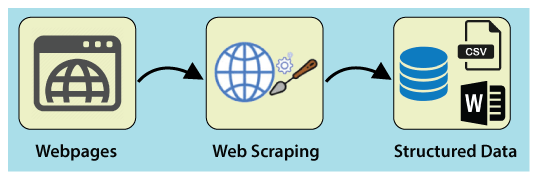
\includegraphics[width=0.7\textwidth]{obrazky-figures/web-scraping-using-python.png}
	\caption{Všeobecný postup, ktorým sa aplikácia typu web scraper riadi. Prevzaté z \cite{WebScrap}.}
	\label{WebScrap_img}
\end{figure}

\bigskip

Medzi najpopulárnejšie web scrapery patria aplikácie s jednoduchou point-and-click politikou. Po inštalácii takejto aplikácie používateľ jednoducho zvolí webové dokumenty, z ktorých chce extrakciu prevádzať a následne interaktívne vyznačí dáta, ktoré ho zaujímajú. Pre používateľov, ktorí nemajú príliš veľké skúsenosti s informačnými technológiami a nechcú platiť za túto službu nemalé peniaze rôznym korporáciám, je to skrátka jediná možnosť \cite{scrapers}.

\bigskip

Spomínaný prístup má samozrejme svoje výhody, medzi ktoré sa radí najmä spomínaná používateľská prívetivosť a relatívne nízka cena, avšak v prípade potreby automatizácie takejto činnosti existujú na trhu lepšie riešenia. V prípade, že je potrebná vysoká automatizácia alebo sa jedná o veľké množstvo dát a stránok určených na extrakciu, je výhodnejšie použiť aplikáciu ladenú skôr na tento spôsob. Pri firmách, ktoré sa venujú extrahovaniu údajov z webových stránok na profesionálnej úrovni, sa počet prenesených dát v súčasnosti pohybuje už v petabajtoch. Počet extrahovaných webových stránok sa pohybuje v~miliardách mesačne na jednu takúto firmu \cite{JanCurna:online}.

Pri takto veľkých číslach narážajú spomínané firmy na rôzne problémy, ktoré rádový používateľ web scrapingovej aplikácie riešiť nemusí. Medzi takéto problémy sa radia v neposlednom rade napríklad:
\begin{itemize}
    \item náročnosť na hardvérový čas,
    \item limitovanie počtu možných GET dotazov,
    \item veľká diverzifikácia architektúry webových stránok,
    \item objem dát potrebný na prenesenie údajov a následné uloženie extrahovaných údajov.
\end{itemize}

Spôsobov ako sa takýmto problémom brániť alebo im priam predchádzať, je v dnešnej dobe už viacero. V prípade limitovania počtu možných GET požiadaviek na jednu webovú stránku, je napríklad možné meniť IP adresy, z ktorých sú GET požiadavky odosielané. Ani to však nieje považované za optimálne riešenie. Stránky v dnešnej dobe môžu využívať rôzne ochrany proti web scrapingu, ako napríklad priamu detekciu človeka od robota alebo tzv. CAPTCHA\footnote{Completely Automated Public Turing test to tell Computers and Humans Apart.} \cite{JanCurna:online}.

Web scraping má teda svoje výhody, ale aj nevýhody. Tieto sú popísané podrobnejšie v nasledujúcej časti tejto kapitoly.

\section{Výhody, nevýhody a využitie web scrapingu}

Web scraping má v súčasnosti viac možností a oblastí využitia, ako tomu bolo v minulosti. Toto je dané hlavne neustálim rozširovaním sa internetu ako celku. V počiatkoch internetu sa aplikácie typu web scraper nazývali skôr \textit{crawler} a využívali sa prevažne na indexáciu obsahu a nie na zber, extrakciu a analýzu dát tak, ako je tomu teraz. 

Web scraper je ale aplikácia, ktorá je založená presne na tých fundamentálnych základoch ako spomínaný crawler. Avšak s jediným rozdielom. Jeho úlohou je zber dát. Takýto zber môže prebiehať napríklad kopírovaním dát do databázy. V mnohých prípadoch sú aplikácie typu scraper využívané veľkými korporáciami ako napríklad Microsoft, Amazon alebo Google. Ich účelom je prevažne cielenie zobrazovaných reklám tak, aby boli pre používateľa ako jednotlivca relevantné \cite{online:how_does_scraping_work}.

\bigskip

Jednotlivé prípady využitia takejto aplikácie sa neustále rozširujú, obecne ale platí, že jeho využitie spadá do nasledovných kategórií \cite{WebScrap}:

\begin{itemize}
    \item monitorovanie ceny produktov,
    \item získavanie údajov o nových produktoch na trhu,
    \item analýza konkurencie,
    \item evidovanie údajov o konkrétnej doméne,
    \item monitorovanie ceny leteniek.
\end{itemize}

A mnohé ďalšie prípady. Údaje extrahované touto metódou môžu byť následne využité na širšie pochopenie vývoja udalostí, napríklad na trhu alebo u konkurencie.

Web scraping má teda jasné výhody čo sa kolekcie dát týka. Patria medzi ne už spomínané monitorovanie konkurencie, cien produktov a analýza rôznych dát. V neposlednom rade ale treba poukázať aj na výhody z pohľadu technológie samotnej. Medzi ne patria napríklad:

\begin{itemize}
    \item rýchlo sa rozvíjajúce technológie,
    \item automatizovanie monotónnych činností,
    \item zber obsiahleho množstva dát, ktorý by bol manuálne nemožný,
    \item v porovnaní s manuálnym zberom dát exponenciálne rýchlejšie výsledky.
\end{itemize}

Každá technológia a jej využitie má však aj svoje nevýhody. Manuálny zber dát môže byť taktiež rozumná možnosť, a to hlavne v prípade, že sa jedná o ojedinelú prípadne unikátnu udalosť. V takomto prípade sa tvorba alebo priame využitie web scrapera neodporúča. A~to hlavne pre časovú zložitosť nielen naprogramovania, ale aj samotnej konfigurácie a~zoznámenia sa s aplikáciou. Využitie samostatnej aplikácie na takúto činnosť je rozumné až vtedy, keď sa daná akcia musí opakovať v určitých intervaloch \cite{WebScrap}. 

V takom prípade je potreba zvážiť aj rôzne aspekty v rámci prevádzky, samotnom vytváraní a následnom používaní web scrapera. Medzi najhlavnejšie nevýhody sa preto radí najmä:

\begin{itemize}
    \item nutná znalosť kódu a programovania,
    \item IP Detekcia a CAPTCHA,
    \item ku každej stránke je potreba pristupovať individuálne.
\end{itemize}

Zároveň treba spomenúť fakt, že dynamické stránky môžu často meniť svoju štruktúru. Preto nemôžme zabúdať na údržbu web scrapera nielen z pohľadu úrovne bezpečnosti programu, ale aj z pohľadu údajov, ktoré web scraper prijíma. V prípade, že webová stránka zmení štruktúru tak, že aktuálna konfigurácia web scrapera nedokáže pokračovať v extrahovaní údajov, je potrebné v stránku znova analyzovať. 

Ak web scraper nieje schopný efektívne využiť algoritmy, ktoré v minulosti fungovali, je v niektorých prípadoch potrebné zanalyzovať prístupy web scrapera a upraviť jeho logiku. Bez dodatočného zásahu tak nemusí byť znova funkčný.

\section{Metódy využívané v súčasnosti}

Aktuálne používané metódy sa vo všeobecnosti dajú rozdeliť do dvoch kategórií:
\begin{itemize}
    \item {Pripravené aplikácie}
    \item {Platformy a knižnice}
\end{itemize}

\bigskip

Pripravené aplikácie budú obľúbenejšie najmä pri širokej verejnosti, ktorá má čoraz častejšie o web scraping záujem. Tieto aplikácie predstavujú rýchlu a často jednoduchú cestu k splneniu toho, čo často požadujeme najviac - výsledky rýchlo a kvalitne.

V mnohých prípadoch však chceme priniesť aj svoje nápady na vylepšenia. Nastavenie takýchto aplikácií býva často limitované a ich kód nemusí vždy byť verejne dostupný. V takom prípade je lepšie využiť jednu z dostupných knižníc, na ktorých väčšina týchto aplikácií stavia. 

\subsection{Hotové riešenia}
V prípade, že nás zaujíma len priama extrakcia dát, máme v dnešnej dobe na výber z~mnohých aplikácií. Tie sú pripravené na použitie, a tak nieje treba programovať aplikácie od začiatku. Každá má však svoje vlastné postupy pri extrakcii a z toho plynie fakt, že nie každá takáto aplikácia dokáže splniť požadované zadanie. 

\newpage
Medzi najznámejšie aplikácie v tomto odvetví však patria hlavne \cite{WebScrap}:

\begin{itemize}
    \item {Scrapping-bot}
    \item {Octoparse}
    \item {Import.io}
    \item {Dexi.io}
    \item {Outwit}
\end{itemize}

V niektorých prípadoch nám stačí jednoduché rozšírenie do prehliadača (napr. Web Scraper\footnote{\url{https://webscraper.io/}}), ktoré je samozrejme efektívne hlavne pri menšom počte webových stránok a dát určených na scraping. 

Spomenuté aplikácie sú vo svojom odvetví veľmi populárne, avšak každá z nich má svoje limity. Pre skúsenejších používateľov, ktorí majú záujem web scraping prispôsobiť svojim potrebám, preto žiadna z nich nemusí byť ideálna cesta.

\subsection{Platformy a knižnice}

Pokiaľ však chceme vytvoriť vlastný program alebo aplikáciu typu web scraper, je potrebné rozlišovať na úrovni technológií dostupných pri programovaní. V prvom rade je treba vziať do úvahy programovací jazyk. V takom prípade je na výber rovno z niekoľko voľne dostupných programovacích jazykov. Medzi dva najpopulárnejšie v tomto odvetví však patria hlavne Python a Javascript. Každý má však znova svoje výhody a nevýhody, a preto je treba zvážiť na aké účely bude web scraper používaný. Vo všeobecnosti je využívanejší práve prvý spomínaný Python, vďaka jeho popularite z pohľadu jednoduchosti písania čistého kódu, komunity a podpory, ktorá mu je venovaná. Python ponúka veľké množstvo frameworkov, z ktorých tie najpopulárnejšie zahŕňajú hlavne Selenium\footnote{\url{https://www.selenium.dev/}} a Scrapy\footnote{\url{https://scrapy.org/}} \cite{The5Best}. Tieto som samozrejme zohľadnil pri výbere vhodného frameworku na vytvorenie web scrapera.

Na druhej strane je tu však Javascript, ktorý je vyvíjaný priamo pre prácu s webovými stránkami. Kým Python je lepší čo sa týka podpory a rozšírenosti frameworkov, Javascript má výhodu v lepšej integrácií nielen s webovými stránkami, ale aj s webovými prehliadačmi samotnými. Python v mnohých prípadoch vyžaduje špeciálny ovládač na komunikáciu s~prehliadačom a podpora dynamických stránok je znova jednoznačne lepšia pomocou Javascriptu. Je to tak práve kvôli jeho spomínanej lepšej integrácií a faktom, že Javascript je jednou z hlavných súčastí dynamických moderných webových stránok. Javascript je jednou z hlavných prvkov modernej webovej stránky, ktorá sa skladá ešte z HTML a CSS. Jeho úlohou je hlavne vytváranie dynamického obsahu, ktorý vyvoláva dojem, že webová stránka s užívateľom interaguje. Vo väčšine prípadov beží iba na strane klienta, takže dynamickosť samotná nezaťažuje server. Zároveň je v mnohých prípadoch využívaná asynchrónnosť\footnote{Asynchrónnosť znamená v tomto prípade neblokovanie prostriedkov prehliadača a načítavanie obsahu webovej stránky zároveň so skriptami.} tohto programovacieho jazyka na zlepšenie odozvy a interakcie \cite{Javascript}. Práve tento fakt sa stáva rozdielovým faktorom pri extrakcii dát z webových stránok, keďže obsah webovej stránky sa v mnohých prípadoch môže načítavať asynchrónne a nezávisle od ostatných častí webu. Z môjho vlastného rozboru a výskumu som zistil, že dynamickosť a~asynchrónnosť stránok je prvok, ktorý je lepšie zvládaný za pomoci Javascriptu.

\bigskip

Rozhodnutie používať Javascript som učinil zároveň s predpokladom využitia jedného z jeho voľne dostupných frameworkov. Zároveň som zohľadnil svoje predošlé skúsenosti práve so spomínaným jazykom. K tomuto rozhodnutiu prispel aj fakt, že v dnešnej dobe je dynamika stránok považovaná za štandard a tu hrá úloha Javascriptu veľkú rolu. V procese výberu frameworku som zohľadňoval hlavne integráciu daného frameworku s prehliadačom, výbornú podporu dynamických stránok a podporu asynchrónnosti, ktorá je pri takejto aplikácii kľúčová.

Ako prvý framewrok spomeniem určite Apify SDK, za ktorým stojí česká firma Apify Technologies\footnote{{\url{https://apify.com/}}} \cite{JanCurna:online}. Medzi najznámejšie technológie používajúce Javascript patria určite aj nasledovné:

\begin{itemize}
    \item {Apify SDK}
    \item {Puppeteer}
    \item {Cheerio}
\end{itemize}

Z pomedzi týchto technológií, ktoré zdieľajú niektoré základné funkcie, bola na zostavenie výslednej aplikácie použitá technológia Puppeteer. Puppeteer je zároveň jedna z~technológií využívaných práve spomínanou firmou Apify Technologies. 

V porovnaní s technológiou Cheerio má Puppeteer svoje výhody. V niektorých faktoroch vyhráva aj Cheerio. Preto je treba zvážiť hlavne nasledovné:

\begin{itemize}
    \item možnosť scrapingu dynamických stránok,
    \item funkcionality a možnosti,
    \item kompatibilita webových technológií,
    \item rýchlosť analýzy a extrakcie.
\end{itemize}

V prvom rade treba zvážiť aktuálnu situáciu a technológie, ktoré sa na webe vyskytujú. 95\% webových stránok v súčasnosti používa Javascript, takže predpoklad, že moderné weby budú obsahovať dynamický obsah je prevažne jasný, a preto treba s takýmto obsahom počítať. Node.js, ktorý je postavený na Javascripte, je zároveň najrýchlejšie sa rozširujúcou nielen webovou technológiou. V čase písania má Node.js viac ako 1,5 milióna dostupných rozširujúcich balíčkov a jeho náskok je v súčasnej dobe jednoznačný \ref{Moduleco_img} \cite{HowPopular}. 

\begin{figure}[hbt]
	\centering
	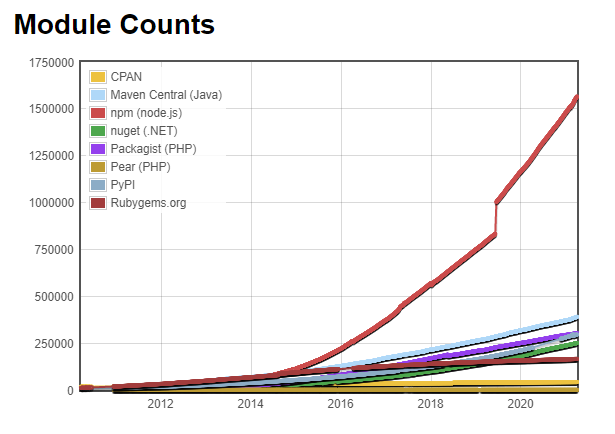
\includegraphics[width=0.7\textwidth]{obrazky-figures/modules.png}
	\caption{Porovnanie najpopulárnejších technológií a vývoj počtu ich modulov. Prevzaté z~Moduleco \url{http://www.modulecounts.com/}, citované 30.3.2021.}
	\label{Moduleco_img}
\end{figure}

\bigskip

Pri porovnávaní technológií Puppeteer a Cheerio je na prvý pohľad jednoznačné, čo majú spoločné a v čom naopak každá z nich vyniká. Tieto poznatky pomôžu určiť výslednú technológiu na základe požiadaviek, ktoré vznikli zároveň s výberom témy tejto práce.

Cheerio a Puppeteer sú technológie založené na Node.js a patria medzi najpopulárnejšie technológie v tomto odvetví. Ich jednoznačné vlastnosti však definujú nielen ich možné prípady použitia, ale zároveň schopnosti a rýchlosť, akou sú schopné dosiahnuť očakávané výsledky. 

\newpage

Puppeteer je technológia, ktorá je vyvíjaná za účelom automatizácie webového prehliadača, zatiaľčo hlavným určením Cheeria je web scraping samotný. Cheerio nespolupracuje so žiadnym webovým prehliadačom. Jednoducho vytvorí HTTP požiadavku na webový server a ten odpovie obsahom v podobe HTML. Tým, že Cheerio je určené priamo na požadovanú úlohu, je v tomto ohľade rýchlejšie a výhodnejšie pre web scraping \cite{cheerio}.

Na druhú stranu Puppeteer je viazaný iba na prehliadač Google Chrome vo forme Chromium. Puppeteer má priamu kontrolu nad prehliadačom, takže je možné ovládať prehliadač ako celok. Tento fakt sa dá brať aj ako výhoda, aj ako nevýhoda, keďže je to pravdepodobne jeden z dôvodov prečo je Puppeteer pomalší vo vykonávaní funkcie Web Scrapera. Puppeteer však prináša schopnosť plynulej práce s Javascriptom na webovej stránke. Dokáže pracovať aj s webovými stránkami postavenými na moderných technológiách ako React alebo Angular, ktoré sú v dnešnej dobe na vzostupe pre ich moderné prvky. Z priamej integrácie s~prehliadačom vyplýva aj fakt, že Puppeteer dokáže vytvárať snímky obrazovky počas načítavania a pracovania s webovou stránkou. Zároveň podporuje technológiu XML a nerobí mu problém ako čítanie, tak ani parsovanie a priame spúšťanie funkcií Javascriptu~\cite{puppeteer},~\cite{cheerio}. 

Práve podpora dodatočných funkcií a možnosť parsovania dynamických stránok s Javascriptom ma presvedčili pre výber technológie Puppeteer. Rozširovaním poznatkov o technológii Puppeteer som si tento pocit presvedčenia len overil. Následne som túto technológiu využil pri návrhu architektúry a implementácii výslednej aplikácie.

\bigskip

Z uvedených informácií je pomerne jasné aké výhody a nevýhody dané riešenia majú a čo ponúkajú. Ako už bolo spomenuté v úvode tejto práce, jej cieľom je zjednotiť hlavne vstupné požiadavky tak, aby sa jednotlivé časti týchto požiadaviek neviazali na jednotlivé webové dokumenty. Popis návrhu je predstavený v nasledujúcej časti tejto kapitoly.

\newpage

\section{Navrhované riešenie}

Táto práca má za úlohu vytvoriť aplikáciu s unikátnymi vlastnosťami umožňujúcimi extrakciu založenú na obsahu webovej stránky. Kľúčové vlastnosti aplikácie budú tvorené hlavne vstupným a výstupným formátom, postupom, ktorý aplikácia bude na extrakciu dát využívať a dôrazom na dodržanie univerzálnosti vstupných pravidiel. 

Univerzálnosť vstupných pravidiel v tomto prípade zabezpečí využiteľnosť raz definovaných požiadaviek na viaceré webové dokumenty a dátové sety. Definícia vstupných pravidiel bude rozdelená na hlavné a vedľajšie pravidlá tak, aby bolo možné odlíšiť vnútornú konfiguráciu aplikácie a používateľské pravidlá za účelom jednoznačne určiť ich prioritu a typ využitia. Vstupné pravidlá nemôžu byť závislé na štruktúre webového dokumentu, ale na jeho obsahu.

Finálna aplikácia bude vyvíjaná pomocou technológie Puppeteer najmä vďaka jeho jednoznačnej integrácií s webovým prehliadačom. To sa na prvý pohľad nemusí zdať dôležité. Jedná sa predsa o aplikáciu na extrakciu dát, nie aplikáciu, ktorá slúži na automatizáciu prehliadača. Údaje z webovej stránky sa dajú získať jednoduchšie, bez využitia webového prehliadača, ktorý celý proces len spomaľuje. 

To je síce pravda, avšak spomínaná podpora dynamických stránok a stránok postavených na moderných technológiách, ako napríklad React a Angular, je značne limitovaná. Načítanie týchto stránok tak, aby ich zobrazenie zodpovedalo realite je prehliadačom Chrome zvládnuté bez akýchkoľvek problémov. Protokol Chrome DevTools dokáže zabezpečiť komunikáciu na vysokej úrovni, ktorá dané dáta prenesie tak, ako bolo zamýšľané. Po nadviazaní spojenia má Puppeteer plnú kontrolu nad prehliadačom a extrakcia dát môže začať. 

Postup, ktorý bude aplikácia na analyzovanie a detekciu obsahu používať, bude popísaný v nasledovných kapitolách. Mal by byť efektívny, s dôrazom na presnosť a rýchlosť akou dokáže rozpoznať, že sa jedná o falošné alebo pravé výsledky. To bude jednoznačne určené porovnaním s definovanými vstupnými pravidlami.

\bigskip

Už samotný protokol DevTools používa technológiu JSON kvôli jeho jednoznačným výhodám v oblasti prenostiteľnosti medzi nielen aplikáciami, ale aj programovacími jazykmi. Komunikácia výslednej aplikácie z pohľadu vstupných a výstupných dát by preto mala tiež využívať práve túto technológiu. Definovanie pravidiel bude v tomto formáte pre človeka jednoduché na zápis a pre stroj jednoduché na čítanie. 

Formát JSON bude zároveň použitý aj na spätnú komunikáciu, kde sa v tomto formáte budú po úspešnom dokončení procesu nachádzať vygenerované výsledky. Tieto výsledky budú tak pripravené na ďalšie využitie v praxi.

Pri návrhu riešenia boli brané v úvahu aktuálne dostupné aplikácie a frameworky. 


\chapter{Technológie}
\label{Technologie}

Táto kapitola sa zaoberá popisom technológií, modulov a prvkov, na základe ktorých bude následne zostavená aplikácia. Ako cieľ je považované dosiahnuť čo najefektívnejšie nielen jej využívanie, ale aj jej údržbu. Zároveň treba brať v úvahu aj prívetivosť a jednoduchosť používateľského vstupu, jeho formát, využiteľnosť a prenositeľnosť výstupných dát. 

K výberu týchto technológií boli využité poznatky z Kapitoly \ref{aktualny_pristup}, ktoré ďalej určovali smer návrhu a vývoja aplikácie.

\section{HTML}

Základným stavebným blokom každej webovej stránky je nepochybne HTML. HTML je skratka pre \textit{HyperText Markup Language} a už svojím názvom napovedá, akú úlohu vo webových technológiách zohráva. 

HTML dokument sa skladá z elementov, ktoré sú predstavené v podobe takzvaných \textit{značiek}. Tieto značky sú reprezentované pomocou znakov \textit{<>}. Tie nám dovoľujú určovať typ a rozsah uvedeného obsahu. Tieto elementy môžu obsahovať zároveň rôzne ďalšie atribúty, ako napríklad trieda elementu alebo identifikátor. Takéto atribúty sú potom využívané v~technológiách, ktoré s HTML dokumentami spolupracujú, ako napríklad CSS a Javascript.

Takéto dokumenty sú následne reprezentované vo webovom prehliadači. Ten HTML dokumenty zobrazí zároveň s doplnkovými dokumentami, ktoré určujú štylizáciu a správanie sa danej webovej stránky. HTML dokumenty samotné neobsahujú žiadnu štylizáciu, avšak typ použitého elementu je kritický. To hlavne z dôvodu, že udáva základné rozloženie obsahu, ktorý element predstavuje \cite{WhatisHTML}.

\section{DOM}
\label{DOM}

Jazyk HTML nieje určený na programovacie účely, a preto je potrebné pri práci s webovými stránkami zvážiť aj technológiu DOM. DOM je skratka reprezentujúca \textit{Document Object Model}. Predstavuje akési prepojenie medzi HTML a programovacím jazykom, ktorý chce s webovou stránkou komunikovať \cite{DOM}.

Pri komunikácií s programovacím jazykom DOM reprezentuje stránku v dvoch hlavných podobách:

\begin{itemize}
    \item {Uzly}
    \item {Objekty}
\end{itemize}

Práve tento fakt nám ďalej dovoľuje s webovou stránkou interagovať a meniť jej obsah. Príkladom takéhoto využitia je jazyk Javascript, ktorý bol vyvinutý za účelom vytvorenia dojmu interakcie používateľa s webovou stránkou. 

DOM je zároveň veľmi dôležitý pri web scrapingu. Práve komunikácia s webovou stránkou na úrovni programovacieho jazyka je kľúčová pri extrahovaní požadovaných údajov z webových dokumentov. Takáto extrakcia je možná vďaka reprezentácií webovej stránky v~objektovo orientovanej podobe.

\section{CSS}

CSS predstavuje istý jazyk, ktorý je používaný za účelom popisu štylizácie HTML dokumentov. CSS znamená \textit{Cascading Style Sheets}, kde Cascading predstavuje jedno z hlavných pravidiel tohto jazyka - štylizačné pravidlá majú určenú prioritu, podľa ktorej budú aplikované. Tieto pravidlá zároveň umožňujú na jednej webovej stránke používať viacero CSS súborov. 

Primárne určenie je už spomínaná štylizácia a definovanie rozloženia elementov na webovej stránke. Zároveň môžu definovať vzhľad v závislosti od zariadenia, ktoré webovú stránku v danom momente navštívilo. Popisuje teda stav elementov pre médium, na ktorom je webový dokument zobrazovaný \cite{CSS}. 

HTML samotné nebolo vyvinuté za účelom definovania vzhľadu, a preto bolo nutné vyvinúť technológiu, ktorá tento nedostatok kompenzovala. CSS pravidlá sú zväčša aplikované na atribút triedy, ktorý bližšie špecifikuje skupinu prvkov v HTML dokumente. V~niektorých prípadoch sa však pravidlá aplikujú aj na celé elementy, prípadne identifikátory.

Pri vytváraní CSS pravidiel rozlišujeme 3 hlavné miesta, kde sa tieto pravidlá môžu nachádzať:

\begin{itemize}
    \item {Riadkové}
    \item {Interné}
    \item {Externé}
\end{itemize}

Rozlišovanie medzi týmito typmi je dôležité, pretože každé miesto môže mať inú prioritu finálneho vykonania daného pravidla. Výsledná aplikácia využíva fakt, že atribúty triedy sú zväčša používané práve na štylizáciu a tým zaradenie jednotlivých prvkov do jedného logického celku. Tieto celky sa následne dajú využiť na určenie a následnú extrakciu relevantných údajov.

\section{Javascript}

Programovací jazyk Javascript bol vyvinutý za účelom vytvárania dojmu interakcie pri webových stránkach a vývojom rôznych aplikácií. Javascript je jednou z hlavných súčastí webových stránok a je používaný na viac ako 95\% stránkach celosvetovo \cite{HowPopular}. Dá sa preto predpokladať, že jeho integrácia s webovými prehliadačmi a webovými stránkami bude na vysokej úrovni. 

\bigskip

Práve kombinácia HTML, CSS a Javascriptu totiž dokáže docieliť výsledky, aké sa pri moderných štandardoch vyžadujú \ref{Jsexecution_img}. Či už sa jedná o dynamickú zmenu obsahu alebo animovanie niektorých elementov, je to práve Javascript, ktorý túto interakciu docieľuje~\cite{Javascript}. 

\newpage
\begin{figure}[hbt]
	\centering
	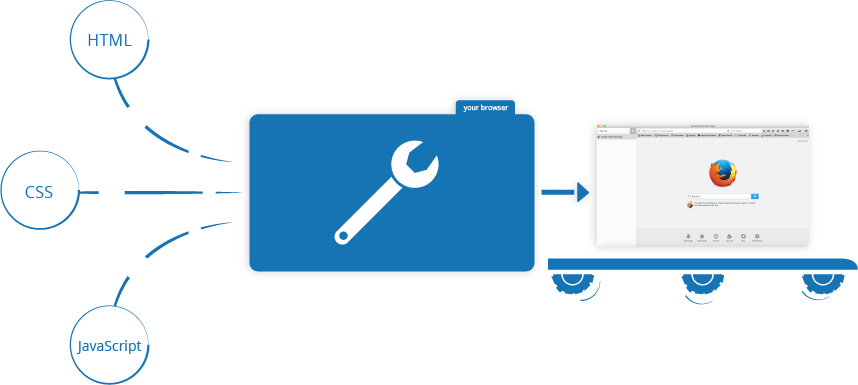
\includegraphics[width=0.8\textwidth]{obrazky-figures/jsexecution.png}
	\caption{HTML, CSS a JavaScript sú 3 hlavné zložky, ktoré spolu vytvárajú web ako ho poznáme dnes. Prevzaté z \cite{Javascript}.}
	\label{Jsexecution_img}
\end{figure}

\bigskip

Javascript je založený na programovacom jazyku Java, ktorý bol ďalej modifikovaný a prispôsobený na prácu priamo vo webovom prehliadači. Javascript dokáže nielen reagovať na vstupy od používateľa, ale reagovať aj na niektoré udalosti na pozadí, napríklad v~prehliadači \cite{Javascript}. 

Táto technológia ďalej stavia aj na asynchrónnosti, teda prístupu za behu. To dovoľuje stránkam načítať Javascript až po načítaní webového obsahu tak, aby nevznikali zbytočne dlhé čakacie doby na načítanie webovej stránky. Zároveň sa dá asynchrónnosť využiť pri odosielaní formulárov, kde nieje nutné po odoslaní znova načítavať stránku. Tým sa zároveň zlepšuje responzívnosť, keďže nie je nutné čakať na vykonanie špecifickej akcie. 

Jednou z najpopulárnejších vlastností tohto programovacieho jazyka je podpora API\footnote{Application Programming Interfaces}. Podpora API umožňuje využitie naprogramovaných rozhraní bez toho, aby si tieto rozhrania používateľ programoval sám. Tento fakt urýchľuje vývoj webových aplikácií a pomáha udržiavať štandard. API pri Javascripte sa primárne rozdeľujú do dvoch kategórií:

\begin{itemize}
    \item {API prehliadača}
    \item {Externé API}
\end{itemize}

Kde API prehliadača predstavuje napríklad aj spomínaný DOM. Ten Javascriptu poskytuje HTML elementy vo forme objektov, s ktorými Javascript dokáže pracovať. Čo sa externých API týka, sem patria najmä API tretích strán, ako napríklad Google Maps alebo Twitter.

V mnohých prípadoch sú to práve API, ktoré môžu naraziť na väčšie množstvo problémov pri načítavaní webovej stránky. Prispieva k tomu aj asynchrónnosť, kde v prípade, že sa HTML dokument načíta skôr ako súborý Javascriptu, môže nastať problém. Vykonávanie skriptu v takom prípade zlyhá. Asynchrónnosť zároveň súvisí s postupnosťou vykonávania kódu. Ak je využitá asynchrónna funkcia, jej výsledok je reprezentovaný v podobe \textit{Promise}. Výsledok Promise nemusí byť dostupný okamžite, a preto v prípadoch, že sa na túto skutočnosť neberie ohľad, môže vykonávanie funkcie zlyhať \cite{Javascript}.

\newpage
\subsection{JSON}

JSON je skratka pre \textit{JavaScript Object Notation}, kde už z názvu vyplýva jeho pôvod. Je to jednoduchá forma popisu objektov tak, že je vo výsledku ľahko čitateľná človekom a~zároveň jednoducho čitateľná počítačom. Aj keď je súčasťou názvu \textit{Javascript}, JSON je univerzálny spôsob zápisu objektov a je to formát adaptovaný mnohými programovacími jazykmi súčasnosti. Práve tieto vlastnosti robia z tohto formátu multiplatformný spôsob prenosu informácií. Podporuje reprezentáciu objektov, čísiel, reťazcov a mnohých ďalších dátových typov. Tieto môže zároveň ukladať do polí a vytvárať tak skupiny. Všetky spomínané štruktúry sú podporované modernými prehliadačmi a programovacími jazykmi, ktoré sa v tomto zmysle používajú. JSON sa najčastejšie používa pri Javascriptových a webových aplikáciách \cite{JSON}.

\subsection{Node.js}

Node.js ako behové prostredie Javascritu bolo vytvorené hlavne za účelom obsluhovania asynchrónnych aplikácií. Beží na Javascriptovom rozhraní V8, ktoré bolo pôvodne vytvorené pre webový prehliadač Google Chrome. Práve vytvorenie tohto rozhrania viedlo k~neskoršiemu vytvoreniu Node.js. Toto rozhranie dokázalo urýchliť Javascript kód pomocou priamej interpretácie kódu do jazyku počítača. Node.js predstavoval možnosť spúšťania Javascript kódu mimo webového prehliadača priamo na fyzickom počítači. To viedlo k~vytváraniu aplikácií priamo spustiteľných či už na počítači alebo smartfóne. Neskôr sa pridali rôzne moduly, ako napríklad HTTP. Tie umožňovali ďalšie rozšírenie pôsobenia, a to napríklad aj na servery tak, aby mohol Node.js pôsobiť ako samostatné prostredie na strane servera. Node.js je v dnešnej dobe využívané zároveň pri rôznych moderných technológiách, ako napríklad React a Angular. Tieto technológie predstavujú frameworky založené a fungujúce práve vďaka Node.js \cite{Node}.

\bigskip

Node.js ponúka zároveň možnosť využitia rôznych modulov. Moduly boli vyvinuté za účelom rozšírenia vlastností a funkcionality. Aj vďaka týmto modulom a faktu, že s ich príchodom je možné Javascript využívať ako na backende, tak aj na frontende, sa Javascript stáva viac a viac populárnym. O tom svedčia aj jeho štatistiky z pohľadu vývoja týchto modulov. Moduly sú ďalej pre používateľov distribuované pomocou NPM.

\subsection{NPM}

Jednou z najdôležitejších súčastí Node.js je NPM(Node Package Manager). Jedná sa o~najväčšie a najpopulárnejšie úložisko doplnkových modulov a projektov pre Node.js. Jeho popularita stále stúpa a aktuálne sa v ňom nachádza už viac ako 1,5 milióna rôznych projektov \ref{Moduleco_img}. Je používaný na zdieľanie nielen open-source projektov, ale aj interných projektov rôznych korporácií. Inštalácia aplikácií a modulov je jednoduchá aj napriek jeho rôznym možnostiam. Zároveň poskytuje jednoduchý spôsob udržiavania aplikácií a ich aktualizácie. Rozšírenosť a jednoduchosť používania poskytuje možnosť rýchlej prenositeľnosti vytvorenej aplikácie \cite{npm}. A práve tu sa nachádza aj knižnica Puppeteer.

\newpage
\subsection{Puppeteer}

Hlavnou súčasťou výslednej aplikácie je Puppeteer. Je to jedna z mnohých knižníc vytvorených pre Node.js distribuovaná pomocou NPM. V aplikácií zohráva dôležitú úlohu, keďže práve technológia Puppeteer je spôsob akým aplikácia komunikuje a extrahuje údaje z prehliadača \ref{pupepyramid_img}. 

Spojenie s prehliadačom je nadviazané pomocou protokolu DevTools vyvinutého spoločnosťou Google a používa prehliadač Google Chrome alebo Chromium v špeciálnom \texttt{headless} móde, kedy nie je zobrazená vizuálna inštancia prehliadača, avšak všetky ostatné funkcie sú plne dostupné \cite{puppeteer}.  

\bigskip

\begin{figure}[hbt]
	\centering
	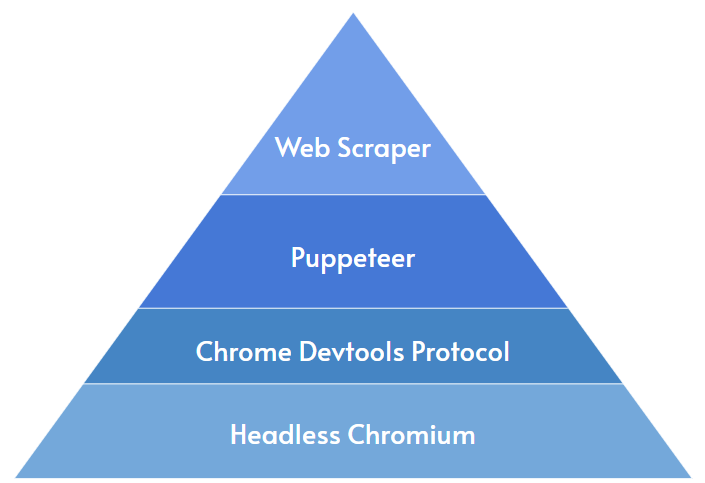
\includegraphics[width=0.6\textwidth]{obrazky-figures/pyramid.png}
	\caption{Hierarchia výslednej aplikácie pri použití technológie Puppeteer. Prevzaté z \cite{pyramid}.}
	\label{pupepyramid_img}
\end{figure}

\bigskip

Z uvedenej hierarchie je na prvý pohľad jasné, na ktorých technológiách Puppeteer stavia:

\begin{enumerate}
  \item \textbf{Headless Chromium} je spôsob spustenia prehliadača Chromium v takzvanom headless prostredí, kedy sa inštancia programu Google Chrome alebo Chromium spustí v režime server bez používateľského prostredia. Ovládanie prehliača je umožnené za pomoci terminálu. Používa sa na rôzne testovanie a automatizáciu. Režime headless je pri používaní Puppeteeru nastavený ako základný, avšak je možné ho vypnúť a~používať Chromium v headfull móde, teda so zobrazeným používateľským prostredím~\cite{chromium}.
  \item \textbf{Chrome DevTools protokol} bol založený za účelom automatizácie prehliadača Google Chrome, Chromium a ostatných webových prehliadačov založených na prostredí Blink. Predstavuje komunikačný prvok medzi programom a webovým prehliadačom. Komunikačné kanály sú rozdelené podľa domén využitia a komunikácia medzi prehliadačom a aplikáciou ďalej prebieha za pomoci formátu JSON \cite{devtools}.
  \item \textbf{Puppeteer} ďalej nadväzuje na protokol DevTools v podobe API, ktoré týmto protokolom dokáže komunikovať s inštanciou prehliadača Chrome.
  \item \textbf{Web scraper} následne využíva knižnicu Puppeteer. Tá prichádza s radom revolučných riešení umožňujúcich automatizovať takmer čokoľvek.
\end{enumerate}

\newpage

Puppeteer bol vytvorený za účelom kompletnej automatizácie prehliadača Chromium. Toto zahrňuje aj zber štatistík o používaní a vykonávaní testov rôznych aplikácií. Niektoré z ďalších prípadných využití tejto knižnice zahŕňajú aj \cite{puppeteer}:
\begin{itemize}
    \item vytváranie snímky obrazovky z webových stránok,
    \item automatizácia formulárov,
    \item vytvorenie testovacieho prostredia pre akúkoľvek aplikáciu.
\end{itemize}

\bigskip

Puppeteer vytvára pomocou protokolu Chrome DevTools komunikačné kanály medzi aplikáciou a webovým prehliadačom. To dovoľuje následnú interakciu s DOM a analýzu webovej stránky. Podporuje sledovanie sieťovej aktivity, vďaka čomu nie je nutné vytvárať explicitné čakacie doby. Táto funkcia je dôležitá pre kompletné načítanie webovej stránky, vrátane asynchrónnych prvkov a externých API. Puppeteer zároveň dokáže čakanie špecifikovať na prítomnosť elementu záujmu alebo na čas, kedy sieťová aktivita webovej stránky klesne na určitý počet požiadaviek za sekundu.

Online verzia Puppeteeru je zároveň dostupná v sandbox prostredí\footnote{\url{https://try-puppeteer.appspot.com/}}, za účelom jednoduchého vyskúšania jeho možností.

\bigskip

\begin{figure}[hbt]
	\centering
	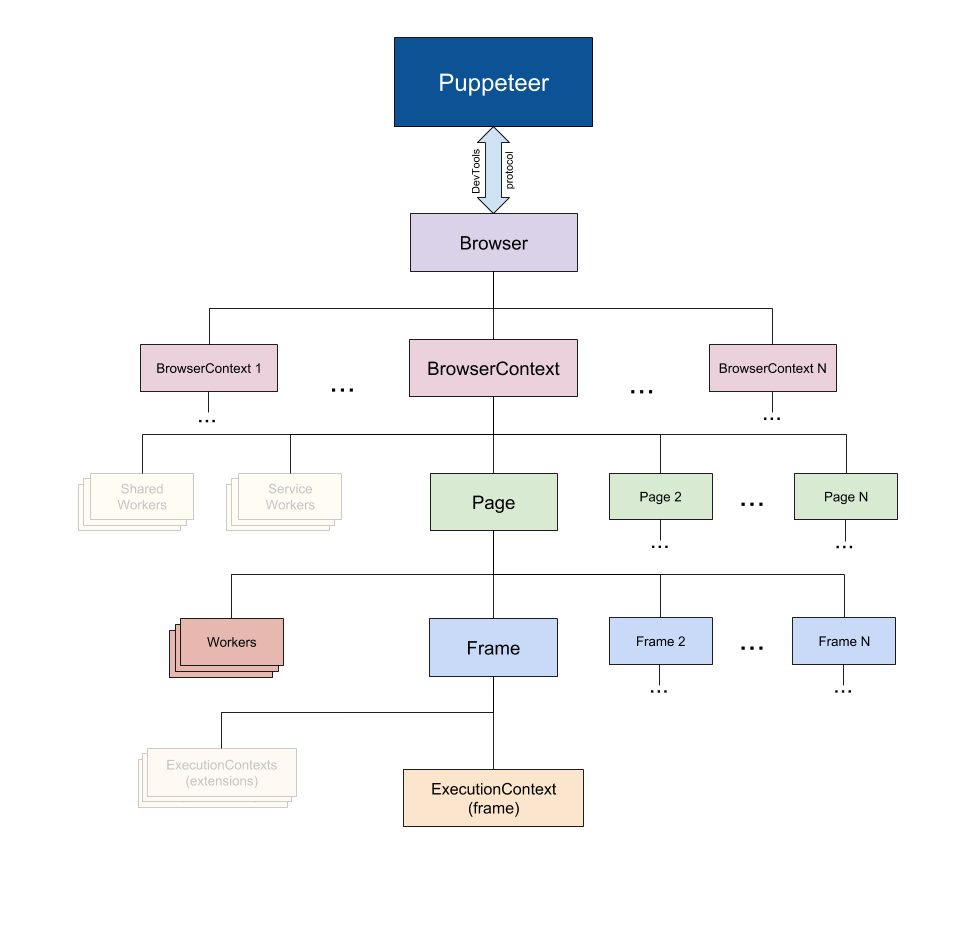
\includegraphics[width=1\textwidth]{obrazky-figures/diagram.png}
	\caption{Diagram knižnice Puppeteer zobrazujúci vzťah jednotlivých prvkov API. Prevzaté z \url{https://github.com/puppeteer/puppeteer/blob/main/docs/api.md}.}
	\label{diagram}
\end{figure}

Vo výslednej aplikácii je Puppeteer využívaný v rámci hlavného procesu, kde sa ako prvé vytvorí inštancia Puppeteeru za pomoci príkazu \texttt{await puppeteer.launch();}. Nasleduje vytvorenie inštancie stránky vo webovom prehliadači za pomoci ďalšieho príkazu \mbox{\texttt{await browser.newPage();}}. Vzniknutá stránka slúži ako prostredie pre načítanie a následnú extrakciu dát z jednotlivých webových stránok. Knižnica Puppeteer obsahuje širokú škálu funkcií. Tie dovoľujú komunikovať s prehliadačom obojsmerne, a teda prijímať aj odosielať dáta prehliadaču. Bezproblémová komunikácia medzi aplikáciou a prehliadačom je základom pre úspešnú interakciu a extrakciu dát. Nasledujúci diagram \ref{diagram} predstavuje vzťah jednotlivých prvkov knižnice Puppeteer a spôsob akým komunikuje.

Všetky vlastnosti a výhody Puppeteeru boli zvážené v rámci návrhu architektúry aplikácie.

\chapter{Návrh architektúry aplikácie}
\label{Navrh}
Úlohou tejto kapitoly je oboznámenie s návrhom architektúry finálnej aplikácie. Architektúra sa skladá z definovania požiadaviek na vstupné dáta, výstupné dáta a vnútorné chovanie aplikácie. V úvahu je samozrejme braná aj aktuálna situácia a stav dostupných riešení.  S tým je spojená aj analýza, ktorá určovala smer vývoja pri dôležitých otázkach ohľadne vnútornej štruktúry aplikácie.

\section{Špecifikácia požiadaviek}

Ako už názov práce predpovedá, jedná sa o extrakciu dát z webových stránok. Avšak dáta sa z webových stránok dajú extrahovať mnohými spôsobmi. Tie však nie sú ekvivalentné. A to nielen z pohľadu presnosti, ale aj z pohľadu rýchlosti extrakcie, spôsobu extrakcie a~ďalších aspektoch viazaných na logiku zvolenej aplikácie.

Základom extrakcie je zároveň vedieť, o aké dáta máme záujem. Tieto dáta teda musia byť jednou z hlavných častí definovaných na vstupe aplikácie. To v akom formáte, a v akej podobe budú tieto dáta reprezentované, bude popísané v nasledujúcich častiach tejto kapitoly. Už teraz je však isté, že pre dosiahnutie pomerne vysokej presnosti bude potrebná špecifikácia rôznych pravidiel. Tieto pravidlá potom budú udávať mernú jednotku na porovnávanie nájdených potencionálnych výsledkov s definovanými pravidlami.

Úlohou týchto pravidiel bude určenie relevantnosti nájdených dát. Aplikácia bude preto tieto vstupné pravidlá overovať z pohľadu správnosti formátu. Pri definícií týchto pravidiel bude treba zohľadniť diverzitu a premenlivosť hľadaného objektu, ako napríklad premenlivú dĺžku reťazcov. Dá sa teda s určitosťou predpokladať, že správna definícia vstupných pravidiel bude mať jednoznačný vplyv na úspešnosť výsledkov z hľadiska nášho očakávania. Preto je treba tomuto návrhu venovať dostatočne veľký časový priestor.

Pri návrhu je treba samozrejme zohľadniť fakt, že finálny používateľ bude chcieť špecifikáciou týchto pravidiel stráviť čo najmenej času. To je samozrejmé. Preto je dôležité odlíšiť dva typy pravidiel. Niektoré pravidlá nie je nutné prepisovať tak často, iné sa môžu meniť s príchodom nových požiadaviek.

Po zadefinovaní vstupných pravidiel bude možné odlíšiť irelevantný obsah od toho, ktorý nás zaujíma. Vo výstupnom súbore by sa mali nachádzať iba údaje užitočné pre koncového užívateľa. Tie budú korešpondovať práve so zadefinovanými pravidlami tak, že práve tieto pravidlá budú slúžiť ako nielen možnosť kontroly údajov, ale aj ako štruktúra výstupného súboru. 

\newpage
\section{Vstupné pravidlá}

Pojmom vstupné pravidlá rozumieme pravidlá, ktoré sú definované ako základné vstupné údaje pri spustení aplikácie. Tieto údaje budú mať za úlohu definovať presne to, čo v danom konkrétnom prípade používateľ aplikácie očakáva ako aplikačný výstup. Sú to zároveň pravidlá pre aplikáciu, určujúce objekty vo webovom dokumente, ako bod záujmu extrakcie pri konkrétnej extrakčnej úlohe. 

Diagram \ref{rules} reprezentuje postup analýzy a zaradenia elementu. Po extrakcii potencionálnych výsledkov je potrebná ich analýza a zaradenie. Výsledky sú na základe ich polohy v rámci DOM zlúčené do kandidátnych skupín. Jedna skupina tak pozostáva z reťazcov znakov jednotlivých DOM elementov. Každý reťazec je analyzovaný zvlášť a pri analýze je overená platnosť definovaných pravidiel. Ak reťazec splní jedno z definovaných pravidiel, toto pravidlo určí jeho finálnu príslušnosť v rámci výsledného objektu. Táto príslušnosť pozostáva zo zaradenia dátového typu a finálneho identifikátora v rámci výsledného objektu. Výsledný objekt reprezentuje objekt, ktorý je zaradený do skupiny objektov určených na zápis do výstupného súboru.

Ako formát týchto pravidiel bol vybraný už spomínaný JSON, vďaka jeho jednoduchej zrozumiteľnosti ako z pohľadu človeka, tak aj z pohľadu počítača. Súbory vo formáte JSON sú zároveň veľmi jednoducho prenositelné aj medzi viacerými programovacími jazykmi, čo je samozrejme ďalšia výhoda. S týmto formátom mám zároveň osobné skúsenosti, takže to bola pomerne jasná voľba.

\bigskip

\begin{figure}[hbt]
	\centering
	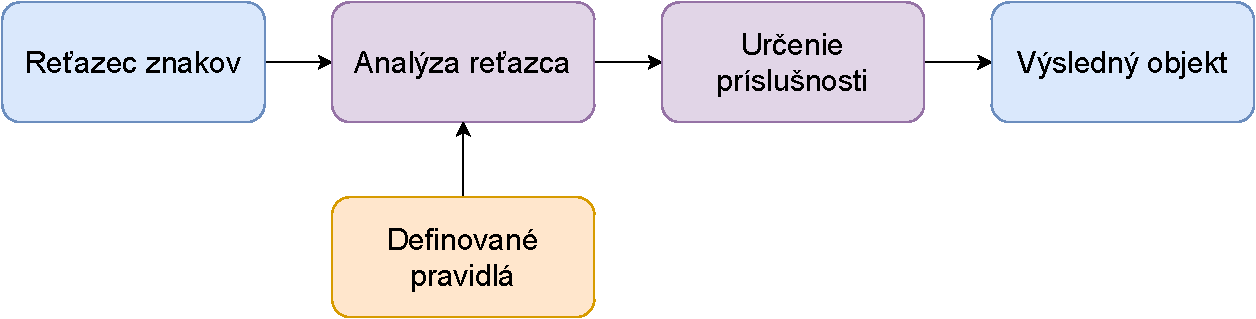
\includegraphics[width=0.9\textwidth]{obrazky-figures/rules.pdf}
	\caption{Spôsob určenia finálneho dátového typu a príslušnosti objektu}
	\label{rules}
\end{figure}

\bigskip

\subsection{Hlavné pravidlá}

V prvom rade treba začať návrhom toho, z čoho sa vlastne tieto vstupné pravidlá budú skladať. S ohľadom na jednoduchosť definovania týchto pravidiel používateľom, boli hlavné a vedľajšie pravidla rozdelené. Rozdelenie konfiguračných a vstupných pravidiel uľahčí ich nasledovnú správu a zaradenie. Príklad štruktúry hlavných pravidiel je zobrazený aj ako výpis \ref{data_ex}.

Medzi hlavné pravidlá na extrakciu boli vybrané:
\begin{itemize}
    \item zoznam webových stránok v podobe URL,
    \item štruktúra hľadaných prvkov,
    \item voliteľný atribút blacklist.
\end{itemize}

\bigskip

Kde \textbf{zoznam webových stránok} určuje všetky webové stránky určené na extrakciu. Malo by sa jednať o webové dokumenty, prípadne HTML dokumenty, uložené v offline podobe na lokálnom disku. Tento zoznam bude slúžiť ako súbor stránok priradený k danej extrakčnej úlohe a všetky definované pravidlá budú pre tieto stránky rovnaké. 

\bigskip

\textbf{Štruktúra hľadaných prvkov} je definovaná ako objekt určujúci požadovaný výsledný názov elementu a jeho \uv{pseudo} dátový typ. Názov bude použitý pri zápise objektu do výsledného súboru a dátový typ bude použitý za účelom klasifikácie daného prvku. Štruktúra je v podobe objektu, teda jednotlivé identifikátory a dátové typy sú k sebe priradené tak, aby aj pre človeka bolo na prvý pohľad jasné, v akom vzťahu tieto údaje sú.

\bigskip

\textbf{Blacklist} je voliteľný atribút (nemusí byť vo finálnom vstupnom súbore reprezentovaný). Bude sa skladať z reťazcov, ktoré používateľ určí ako nežiaduce. Definovanie Blacklistu bude mať za následok ovplyvnenie aplikácie pri jej rozhodovaní o zaradení jednotlivých prvkov.


\subsection{Vedľajšie pravidlá}

Ako vedľajšie pravidlá boli zvolené také pravidlá, ktorých prenositeľnosť aj medzi rôznymi typmi definovaných domén je pravdepodobnejšia. Preto by nemuselo byť vždy nutné tieto pravidlá meniť. Zmena týchto pravidiel sa teda berie ako menej častá udalosť. Vo väčšine prípadov môže stačiť pri zmene extrakčnej úlohy zmeniť len definíciu hlavných pravidiel. Príklad štruktúry týchto pravidiel je zobrazený aj ako výpis \ref{config_ex}.

Medzi tieto pravidlá boli zaradené:
\begin{itemize}
    \item maximálny pomer zlyhania,
    \item formát,
    \item primárny prvok.
\end{itemize}

\bigskip

Ako \textbf{maximálny pomer zlyhania} bude určený pomer irelevantných prvkov ku všetkým nájdeným prvkom z daného okruhu dát. V prípade, že bude tento pomer vyšší ako táto horná hranica, bude výsledný okruh vyradený. Tento okruh sa bude úzko viazať s definíciou primárneho prvku, pretože bude zložený práve z danej skupiny elementov. 

Ak však príde k splneniu tejto podmienky, bude prvý takýto okruh vybraný ako výsledný. Ten bude následne poslaný na analýzu a definíciu jeho obsahu. 

\bigskip

\textbf{Formát} predstavuje objekt, zložený z názvu definovaného dátového typu a jeho korešpondujúcej reprezentácie v podobe jednoznačného regulárneho výrazu. Priamo naväzuje na hlavné pravidlá, ktoré ho využívajú ako zdroj pre regulárne výrazy hľadaných prvkov. Dá sa predpokladať, že správne definovaný regulárny výraz bude viesť k presnejším výsledkom. 

\bigskip

\textbf{Primárny prvok} je taký prvok, ktorý sa v objektoch určených na extrakciu opakuje, a teda je možné sa na jeho prezenciu spoliehať. Tento prvok je súčasťou hľadaného objektu. Jeho deriváciu je možné nájsť v každom objekte, ktorého obsah chceme extrahovať. 

Aplikácia bude tento prvok používať na prvotnú analýzu webovej stránky. Na základe jeho prezencie je následne posúdené, či daný okruh dát je kandidátom na definíciu výsledných objektov.

\newpage

\section{Výstupný formát}

Čo sa výstupného formátu týka, mal by byť znovu pokiaľ možno v univerzálnom formáte. Keďže sa dá predpokladať, že extrahované dáta budú v prípade potreby použité, je vhodné zvoliť formát podporovaný rôznymi aplikáciami a programovacími jazykmi.

Z toho dôvodu tu bol znovu zvolený formát JSON. Návrh počíta s jedným výstupným súborom pre jednu doménu tak, aby výstupný súbor niesol názov domény, z ktorej extrahované údaje pochádzajú. Umiestnenie týchto výsledných súborov je už však na používateľovi. Pri nešpecifikovaní parametra určujúceho cestu k výstupným súborom, bude použitá základná zložka s názvom \textit{output}.

\bigskip

Štruktúra, v akej budú jednotlivé extrahované objekty reprezentované, je zhodná so štruktúrou definovanou v používateľskom vstupnom súbore. Táto štruktúra je potom zachovaná pre všetky objekty. Ak však jeden z kľúčov daného objektu nie je dostupný alebo nebol extrahovaný, je tento kľúč vynechaný. V niektorých prípadoch sa dátový typ daného prvku nemusí podariť definovať. V takom prípade sa vo výslednom objekte môžu objaviť aj kľúče so špeciálnym názvom \textit{undefined}. Konfigurácia aplikácie však dovoľuje spustenie s~parametrom, ktorý zaručuje odstránenie nedefinovaných prvkov z objektu. Tento kľúč značí prvok, ktorého dátový typ nebolo možné na základe špecifikovaných vstupných požiadaviek definovať, avšak patrí do vyhľadávanej podskupiny.

Formát JSON ako výstupný formát je striktne dodržaný a riadne formátovaný tak, aby bol jednoducho čitateľný aj pre človeka. Bezproblémové využitie dát z takto štruktúrovaného výstupu je preto garantované.

\bigskip

Sekundárnym výstupným súborom sú takzvané metadáta. Sú to dáta, ktoré predstavujú rôzne vlastnosti popisujúce priebeh extrakcie pri spustení aplikácie. Metadáta sú znova pre jednoduchú prenositeľnosť vo formáte JSON a jeho objekty obsahujú tieto údaje:

\begin{itemize}
    \item url adresa webového dokumentu,
    \item počet testovaných okruhov,
    \item odkaz na prvý nájdený objekt v podobe \texttt{document.querySelectorAll},
    \item počet výsledných objektov,
    \item čas potrebný na otestovanie okruhov,
    \item čas potrebný na uloženie výsledkov,
    \item čas potrebný na načítanie webového dokumentu.
\end{itemize}

\bigskip

Tieto metadáta môžu poslúžiť ako kontrola výsledných súborov a porovnanie časov potrebných na vykonanie určitých akcií. Metadáta sú generované pri každom spustení aplikácie a ich obsah je prepisovaný tak, aby obsahoval vždy údaje o poslednom spustení.


\subsubsection{Konzolový výstup aplikácie}

Aplikácia zároveň pri každom spustení a jej behu informuje používateľa o aktuálne prevádzanej akcii. V režime bez vypisovania explicitných informácií aplikácia informuje o začatí exekúcie formou vypísania \textit{Execution stared}.  Po skontrolovaní vstupných údajov informuje o začatí extrakcie vypísaním \textit{BEGIN PRIMARY EXTRACTION}. Následne sa vypisujú aktuálne URL, na ktorých extrakcii sa v danom momente pracuje. 

Na záver aplikácia informuje o úspešnosti extrakcie, o lokácii vygenerovaného súboru s~metadátami a o finálnej dĺžke trvania celého procesu v milisekundách.

V prípade spustenia aplikácie s prepínačom \textit{-v} je na výstup vypísaný podrobnejší obsah. V tomto prípade sa na konzolovom výstupe objavia časy jednotlivých akcií, informácie o~počte výsledných objektov, zoznam testovaných okruhov a identifikácia výsledného okruhu.

\section{Architektúra aplikácie}

V tejto časti práce bude popísaná architektúra aplikácie tak, ako bola aplikácia navrhnutá a odôvodnenie týchto krokov. Nasledujúci diagram reprezentuje finálny návrh architektúry aplikácie a vzťah jednotlivých prvkov.

\bigskip

\begin{figure}[hbt]
	\centering
	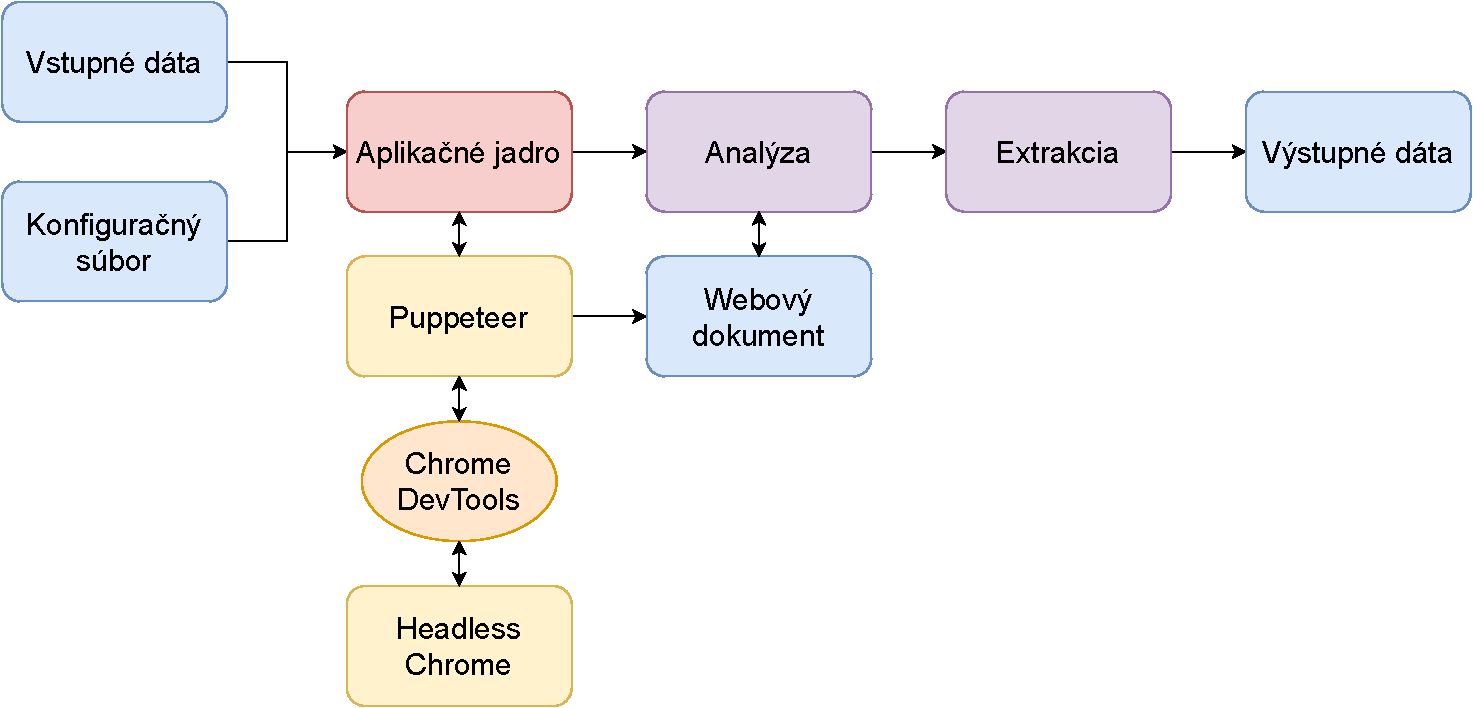
\includegraphics[width=0.9\textwidth]{obrazky-figures/architecture.pdf}
	\caption{Diagram navrhnutej architektúry}
	\label{architecture}
\end{figure}

\bigskip

\subsection{Jadro programu}

Hlavný zdrojový kód sa bude nachádzať v jednom súbore, ktorý pre jednoznačnosť v rámci tejto práce nesie názov \textit{extractor.js}. Koncovka js napovedá, že sa bude jednať o súbor založený na programovacom jazyku Javascript. Pri spúšťaní aplikácie sa preto bude tento súbor volať pomocou príkazu \textit{node}, ktorý značí behové prostredie Node.js.

Aplikácia bude naväzovať na dva prídavné súbory vo formáte JSON, ktoré budú predstavovať vstupné informácie vo formáte popísanom v predošlej časti tejto kapitoly. 

Hlavný komunikačný kanál aplikácie a webového prehliadača bude zabezpečený pomocou technológie Puppeteer a protokolu Chrome DevTools. Toto spojenie bude nadviazané automaticky po spustení aplikácie. Pred nadviazaním tohto spojenia však dôjde ku kontrole vstupných dát zadaných používateľom. V prípade, že je formát vstupných dát poškodený, nie je dodržaná jeho štruktúra alebo vo vstupných súboroch chýbajú niektoré dôležité položky, je o tom používateľ informovaný a vykonávanie je ukončené.

\subsection{Hlavný proces}

Úlohou hlavného procesu bude vymedzenie finálneho okruhu výsledkov. Čo sa týchto okruhov týka, ich proces výberu prešiel rôznymi iteráciami, avšak nakoniec bol zvolený spôsob určovania týchto okruhov na základe atribútu \textit{class}. Aplikácia teda najskôr analyzuje stránku tak, aby bolo možné vygenerovať zoznam používaných atribútov. Na základe tohto zoznamu následne aplikácia generuje výsledné okruhy, naplnené údajmi z daného okruhu definovaného \textit{class} atribútom. 

Aby bolo možné určiť správnosť údajov, je každý údaj porovnávaný zvlášť. Údaje sú porovnávané s reprezentujúcim pravidlom regulárneho výrazu, v tomto prípade primárnym prvkom zo vstupných pravidiel.


\subsubsection{Analýza výsledkov}

Po určení správneho okruhu bude následne aplikácia pracovať s \textit{class} atribútom, ktorý daný okruh dát definuje. Aplikácia berie údaje daného okruhu ako potencionálnu súčasť výsledkov, nemusí to tak ale byť  vždy. Preto aplikácia kontroluje susedné prvky z pohľadu DOM a snaží sa získať čo najviac informácií nielen o susedných, ale aj rodičovských uzloch a detských potomkoch daného prvku.

Po zoskupení týchto informácií a uložení textových reprezentácií týchto prvkov aplikácia prechádza k ďalšiemu kroku, ktorý predstavuje finálnu definíciu \uv{pseudo} dátového typu určeného používateľom.

\bigskip

Položky, ktoré nie je možné definovať vo výsledku používateľovi ani inému programu, ktorý by dáta využíval, nemôžu byť užitočné. Práve z toho dôvodu by mal používateľ týmto prípadom predchádzať a to dvoma spôsobmi. 

Keďže aplikácia analyzuje výsledky ako celok, vie presne určiť, aký dátový typ bol na danom indexe definovaný v predošlých prípadoch objektov, ktorých dáta testom na regulárny výraz prešli. Týmto sa dá jednoducho predísť strate dát pri anomáliách. V niektorých prípadoch však ani toto nie je riešenie. V tom prípade má aplikácia možnosť jednoducho takéto nedefinované výsledky ignorovať a používateľovi vôbec nezobrazovať.

\subsubsection{Generovanie výsledných údajov}

Po analýze výsledkov a ich zaradení k dátovým typom prichádza na rad generovanie výsledných údajov. Aplikácia v tomto prípade generuje výsledky pre každý webový dokument zvlášť. Výsledný súbor následne nesie názov v podobe domény, z ktorej údaje pochádzajú.

Vytvorením výsledného súboru sú analyzované údaje transformované do podoby JSON, ktorý je zároveň riadne formátovaný pre jednoduchú čitateľnosť ako človekom, tak aj počítačom. Akonáhle je generovanie všetkých potrebných dát ukončené, je súbor uzavretý a výsledky sú pripravené na použitie. Pred samotným ukončením aplikácie však prichádza na rad ešte záverečné generovanie metadát, ktorých úlohou je informovať o celkových výsledkoch extrakcie.

Metadáta predstavujú akési dáta o dátach. Ich generovaním dávame používateľovi informácie, ktoré môže pokladať za užitočné. Jasný a jednoduchý prehľad o extrakcii z pohľadu počtu extrahovaných elementov, dĺžky trvania jednotlivých akcií, priebeh analýzy a odkaz na prvý cielený element.

\chapter{Implementácia riešenia}
\label{implementacia}

V rámci tejto kapitoly bude popísaný postup implementácie výsledného riešenia. Aplikácia typu web scraper bude implementovaná na operačnom systéme Windows. Jej využiteľnosť je samozrejme multiplatformná a žiadna z jej súčastí nieje na operačný systém Windows viazaná. Aplikácia bola vo finálnej fáze testovaná aj na operačnom systéme Manjaro, pod ktorým bežala tak, ako bola navrhnutá.

Implementácia bola z pohľadu web scrapingu rozdelená do viacerých častí:

\begin{itemize}
    \item {Konfigurácia}
    \item {Vstupné dáta}
    \item {Jadro aplikácie}
\end{itemize}

\bigskip

Postup práce pri implementácií bol vďaka vytvoreniu návrhu a konzultáciám s vedúcim práce pánom Ing. Radkom Burgetom Ph.D. jednoznačný. Najskôr bola implementovaná aplikačná logika a následne bola táto logika rozvedená. Počas implementácie boli zároveň vyskúšané dva rôzne prístupy k problematike. Tieto prístupy sa týkali hlavne rozlíšenia prístupu k vytváraní dátových okruhov. Po skúmaní som pristúpil k vytváraniu týchto okruhov dát na základe atribútu \textit{class}. Bližšie informácie o tom, ako aplikácia dané okruhy vytvára a analyzuje, budú popísané v rámci tejto kapitoly.

\section{Konfiguračný súbor}

Externá konfigurácia dostupná pre používateľa je uložená v konfiguračnom súbore, ktorý môže používateľ voľne upravovať a dokonca zvoliť svoj vlastný. Základný konfiguračný súbor je k výslednej implementácií pripojený a aplikácia ho očakáva implicitne ako súbor \textit{config.json}.

Jeho úlohou je definícia základných pravidiel, používaných pri extrakcii dát z webových stránok. Formát a obsah tohto súboru je preto jednoznačne daný a musí byť dodržaný. V opačnom prípade hrozí, že aplikácia takýto súbor odmietne a nebude možné v extrakcii dát pokračovať. Aplikácia v takomto prípade používateľa zároveň informuje o danej situácii chybovým hlásením zobrazeným v príslušnom termináli. 
\newpage

\begin{lstlisting}[caption={Príklad konfiguračného súboru},captionpos=b,label={config_ex}]
{
    "maxFailRatio": 70,
    "format":{
        "time": "^(\\d\\d:\\d\\d)$",
        "score": "^(\\d+(\\-|\\:)\\d+)$|^-$|^\\? - \\?$|^\\d\\d$",
        "string": "^[a-zA-Z].*$"
    },
    "primary": "^(\\d+:\\d+)$"
}
\end{lstlisting}

\bigskip

Štruktúra konfiguračného súboru je daná nasledovne:

\begin{itemize}
  \item \textbf{maxFailRatio} ako hodnota v rozsahu 0-100. Táto hodnota definuje maximálny pomer prvkov, ktoré pri určovaní výsledného okruhu neboli úspešné. Tieto prvky sú vo výslednom okruhu dát reprezentované hodnotou \textit{null}. Ak je výsledný pomer týchto prvkov väčší, ako hodnota udaná v \textit{maxFailRatio}, je takýto okruh vyradený a neberie sa pri ďalšom určovaní v úvahu. Táto hodnota je úzko viazaná s hodnotou \textit{primary}, ktorá bude popísaná neskôr. Zmenou hodnoty na číslo blížiace sa 0, dochádza k zväčšeniu výslednej presnosti definície, avšak v mnohých prípadoch môže výsledný okruh so správnymi hodnotami obsahovať takzvané \textit{anomálie}, a preto je vhodné túto hodnotu udávať v rozsahu 30-70. Pri číslach blížiacich sa 100 je znova možné, že výsledný okruh bude \textit{false positive} a nebude možné takýto okruh dát brať ako relevantný.
  \item \textbf{format} predstavuje súbor formátov, na základe ktorých aplikácia definuje dátové typy výsledných prvkov. Tento súbor formátov je definovaný nasledovne:
  
  \textbf{názov\_dátového\_typu : reprezentácia\_regulárneho\_výrazu}
  
  Formáty sú reprezentované ako pravidlá, určené regulárnymi výrazmi. Jeden \uv{pseudo} dátový typ je preto definovaný jedným jednoznačným regulárnym výrazom. Tieto výrazy sú používateľovi prístupné a môže ich definíciu kedykoľvek meniť a pridávať vlastné dátové typy definované vlastnými výrazmi. Ich formát je po takomto definovaní v konfiguračnom súbore dostupný v dátovom súbore na následnú špecifikáciu požadovaných vstupných údajov. Z určenia tohto formátu je možné jednoznačne povedať, že správna definícia týchto formátov bude viesť k úspešnejšej extrakcii. 
  
  \item \textbf{primary} je hodnota regulárneho výrazu, ktorá sa viaže s hodnotou \textit{maxFailRatio} a~to takým spôsobom, že práve táto hodnota je používaná na prvotnú detekciu výsledných dátových okruhov. Tieto okruhy sú definované pomocou atribútu \textit{class}. Jedná sa o hodnotu definovanú používateľom ako primárnu v danom vyhľadávanom prípade. Môže sa jednať napríklad o reprezentáciu skóre pri vyhľadávaní športových výsledkov alebo formát času typický pri daný súbor dát. Primárny prvok môže a nemusí byť súčasťou výsledných údajov.
\end{itemize}

\section{Vstupné dáta}

Aplikácia ďalej potrebuje súbor so vstupnými dátami definovanými používateľom. Tieto dáta sú reprezentované znova vo formáte JSON a dodržanie štruktúry je preto kritické. 

Súbor so vstupnými dátami slúži používateľovi na presnú definíciu danej extrakčnej úlohy. Samostatný súbor je vhodné vytvoriť pre každý súbor domén(skupinu domén, z~ktorej budú následne dáta extrahované) zvlášť. Prípadne je možné meniť vlastnosti a obsah daného dátového súboru tak, aby bol v daný moment jeho obsah relevantný. 

Keďže sa jedná o jeden z primárnych súborov aplikácie, je jeho výskyt podmienený. Aplikácia pomocou neho dokáže určiť, o aké dáta má v danej chvíli používateľ záujem. Tieto dáta budú v rovnakej forme reprezentované vo výstupných súboroch, avšak ich poradie v~rámci výstupného súboru nemusí byť rovnaké.

Formát výstupného súboru je preto so súborom obsahujúcim vstupné dáta úzko viazaný, keďže práve vstupné dáta určujú jeho následnú reprezentáciu. Výstupný súbor dát je založený na formáte JSON a jeho štruktúra odpovedá štruktúre definovanej na vstupe.

\bigskip

\begin{lstlisting}[caption={Príklad súboru so vstupnými dátami},captionpos=b,label={data_ex}]
{
    "urls":[
        "tests/dataset/football/domains/365scores.com.html",
        "tests/dataset/football/domains/777score.com.html",
        ...
    ],
    "structure":{
        "time": "time",
        "team1": "string",
        "score": "score",
        "team2": "string"
    },
    "blacklist":[
        "Canc.",
        "Finished",
        "FRO"
    ]
}
\end{lstlisting}

\bigskip

Vstupné dáta sú formované nasledovne:

\begin{itemize}
  \item \textbf{urls} predstavuje zoznam URL adries webových dokumentov. Tento zoznam je zložený z adries konkrétnych webových dokumentov, o ktorých extrakciu má používateľ záujem. Jeho poradie je pri spustení aplikácie striktne dodržané. Nemalo by však ovplyvniť žiadnu z vlastností aplikácie, pretože aplikácia sa na každý webový dokument pozerá samostatne. V prípade, že sa jedná o webovú stránku stiahnutú do offline podoby, je potrebné určiť absolútnu cestu k danému dokumentu. V takom prípade je zároveň odporúčané aplikáciu spúšťať s parametrom \textit{\texttt{-{}-}offline}. Aplikácia zároveň kontroluje dostupnosť daného webového dokumentu a ak daný webový dokument nie je dostupný, je o tom používateľ riadne informovaný. Zároveň však nie je ukončené vykonávanie programu a aplikácia pokračuje nasledovnými URL adresami zo zoznamu. Toto rozhodnutie bolo učinené hlavne z dynamickej povahy internetu, kde URL adresy sa v mnohých prípadoch môžu často meniť a zastavenie vykonávania programu by bolo príliš obmedzujúce. 
  
  \item \textbf{structure} slúži na definíciu štruktúry extrakčnej úlohy a jej objektov záujmu. Štruktúru definuje používateľ tak, aby odpovedala jeho požadovanému výstupu. Jej formát je definovaný nasledovne:
  
  \textbf{výsledný\_názov : názov\_dátového\_typu}
  
  kde výsledný názov je názov, ktorý používateľ požaduje vo výstupnom súbore a názov dátového typu je \uv{pseudo} dátový typ daného prvku. Dátový typ musí byť zhodný s~jedným z dátových typov v konfiguračnom súbore, v opačnom prípade vyhodnotenie takéhoto prvku nebude umožnené. Počet prvkov v štruktúre nie je obmedzený, avšak jeho štruktúra je obmedzená iba na jednoduché výrazy. Zároveň treba brať na vedomie fakt, že sa jedná o štruktúru objektu, ktorý nás v danej extrakčnej úlohe zaujíma. To znamená, že nemá zmysel do štruktúry zahrnúť iné prvky, ako sú pri danom objekte očakávané.
  
  Vo výslednom súbore sa môžu objaviť len prvky, ktoré tu boli zadefinované. Avšak v~niektorých prípadoch výsledný súbor môže obsahovať prvok \texttt{undefined}. Takýto prvok značí, že sa pri extrakcii dát z daného objektu objavil prvok, ktorý aplikácia nedokázala podľa definovaných pravidiel zaradiť. Tomuto javu sa dá predchádzať spustením aplikácie s parametrom \textit{\texttt{-{}-}noundef}. Pri takomto spustení je každý výsledný objekt kontrolovaný na prítomnosť nedefinovaných prvkov a takéto sú následne z objektu vyradené. Na druhej strane prítomnosť všetkých definovaných prvkov nie je podmienená. Ak niektorý z prvkov pri danom objekte chýba, je jednoducho vynechaný a jeho reprezentácia nie je vo výslednom súbore uvedená ani vo formáte prázdneho reťazca znakov. Takáto situácia môže nastať napríklad pri extrakcii dát z obchodných reťazcov a použitia dátového typu reprezentujúceho \uv{zľavu}. Zľava nemusí byť pri každom produkte určená, a preto aplikácia pri produktoch bez zľavy daný prvok vynechá.
  
  \item \textbf{blacklist} ako voliteľný argument predstavuje zoznam reťazcov znakov, ktoré používateľ rozpoznal ako neočakávané alebo nechcené. V takom prípade používateľ daný reťazec zaradí do zoznamu blacklist, ktorý aplikácií slúži ako zoznam nežiaducich reťazcov. Pri spúšťaní aplikácie je zároveň nutné aplikáciu spustiť s parametrom \textit{\texttt{-}b}. V~opačnom prípade bude blacklist ignorovaný. Pri použití blacklistu nezáleží na tom, či sa daný reťazec znakov nachádza v inom reťazci, existuje ako samostatný reťazec alebo predstavuje jediný obsah daného elementu. V každom prípade je takýto reťazec zachytený a aplikácia ho určí ako prvok na vyradenie z výsledného objektu. Využitie blacklistu je na rozhodnutí používateľa, a preto nie je jeho existencia v súbore so vstupnými dátami podmienená. V prípade ale, že ho používateľ bude chcieť využiť, je treba zachovať jeho jednoduchú štruktúru v podobe poľa reťazcov. Veľkosť poľa nie je obmedzená a môže obsahovať nekonečne veľa výrazov. 
 \end{itemize}
 
 \section{Štruktúra aplikácie}
 
 Výsledná aplikácia je štruktúrovaná do niekoľkých logických častí. Po prvotnom spustení aplikácie prebehne kontrola vstupných parametrov, konfigurácie a vstupných dát. Tým sa zadefinujú vlastnosti programu pri danej extrakčnej úlohe.
 
 Asynchrónny proces následne očakáva vykonanie hlavného procesu. Ten je zložený z~funkcií, ktoré definujú správanie programu. 
 
 Ako prvé aplikácia zabezpečí vytvorenie inštancie API Puppeteer. To znamená, že sa vytvorí inštancia prehliadača Chromium s parametrom \textit{headless}, ktorý prehliadač spustí v špeciálnom móde, kde používateľské prostredie zostáva skryté. Táto forma bola vybraná hlavne kvôli urýchleniu procesu a zachovania jednoty pri vykonávaní danej extrakčnej úlohy. 
 
 Po vytvorení spojenia je vytvorená inštancia pre webovú stránku, ktorá bude v danom bode úlohy analyzovaná. Stránka je následne načítaná a prebehne zber dát v podobe všetkých dostupných triednych atribútov jednotlivých prvkov. Tieto triedne atribúty sú následne zoradené podľa početnosti. Algoritmus následne rozdelí obsah webovej stránky do okruhov, ktoré sú definované práve spomínanými triednymi atribútmi. Tieto triedne atribúty sú viazané na štylizáciu webovej stránky, a preto sa dá určiť, že ich výskyt bude rovnaký pre práve jednu skupinu dát. Zároveň sa dá predpokladať, že ak sa jedná o dáta, ktoré sa na webovej stránke opakujú, tak bude výskyt týchto triednych atribútov väčší ako výskyt iných atribútov. Preto je zoradenie kritické pre rýchlosť analýzy dát. To ako analýza prebieha bude ďalej popísané v tejto kapitole.
 
 Po analýze prebehne extrakcia dát. Tá prebieha v troch krokoch:
 
 \begin{enumerate}
     \item Evaluácia
     \item Klasifikácia
     \item Príprava výsledkov
 \end{enumerate}
 
 \bigskip
 
 Výsledky sú následne pripravené na zápis. Zapísané sú vo formátovanej podobe do výsledného súboru, ktorý nesie názov domény alebo dokumentu, z ktorého boli dané dáta extrahované. Všetky takéto súbory sú následne uložené v preddefinovanej zložke. Ak táto zložka nie je definovaná používateľom, aplikácia zvolí základnú zložku \textit{output} v koreňovom adresári aplikácie. Súbor obsahujúci metadáta je taktiež uložený v koreňovom adresári, avšak mimo zložky s výslednými súbormi. Tým môžeme predísť nesprávnemu zaradeniu metadát a výsledných dát. Používateľ je zároveň o aktuálnej lokácií súboru s metadátami informovaný po skončení vykonávania danej extrakčnej úlohy.
 
 \newpage
 \section{Analýza webovej stránky}
 
 Pre získanie relevantných dát a obsahu z webového dokumentu je potrebné daný dokument analyzovať. Analýza prebieha bezprostredne po načítaní webového dokumentu a je rozdelená do niekoľkých krokov:
 
 \begin{enumerate}
     \item Analýza triednych atribútov
     \item Zoradenie zoznamu tried na základe výskytu
     \item Kontrola daného okruhu dát na prítomnosť primárneho prvku
     \item Overenie pomeru nevyhovujúcich prvkov
 \end{enumerate}
 
 \bigskip
 
 \begin{figure}[hbt]
	\centering
	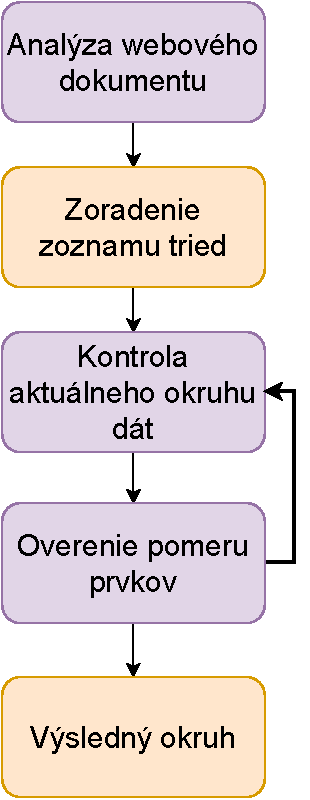
\includegraphics[width=0.3\textwidth]{obrazky-figures/analysis.pdf}
	\caption{Postup pri analýze webového dokumentu}
	\label{analysispdf}
\end{figure}

\newpage

\subsubsection{Analýza triednych atribútov}

Ako prvý krok pri získavaní relevantných údajov o architektúre webovej stránky prebehne analýza triednych atribútov. Aplikácia analyzuje každý prvok reprezentovaný HTML značkou a uloží zoznam všetkých použitých tried, ktoré daný prvok obsahuje. Týmto spôsobom prejde aplikácia všetky značky a získa tak prehľad o všetkých triednych atribútoch na celej webovej stránke.

Keďže sa dá predpokladať, že pri extrakčnej úlohe sa bude zväčša jednať o údaje, ktoré sa na webovej stránke opakujú, sú všetky triedy zoradené do poľa na základe početnosti. Najpočetnejšie triedy budú na vrchole zoznamu a tie, ktoré sa na webovej stránke vyskytujú najmenej, budú na jeho konci. Z toho ako fungujú triedne atribúty pri HTML značkách vieme určiť, že pre jednu skupinu prvkov, ktorá je definovaná jednou spoločnou charakteristikou, budú triedne atribúty spoločné. 


\subsubsection{Zber údajov}

Po zoradení triednych atribútov aplikácia začína so zberom údajov. Postupne od najpočetnejšieho atribútu (toho s najčastejším výskytom) sú dáta, v danom okruhu určenom práve triednym atribútom, uložené a následne kontrolované z pohľadu výskytu primárneho prvku. V prípade, že niektorý z prvkov danej skupiny nepredstavuje primárny prvok, je hodnota daného prvku zmenená na špeciálnu hodnotu \textit{null}. Táto kontrola prebieha porovnaním daného prvku s regulárnym výrazom pre primárny prvok. Hodnota \textit{null} pri určitom prvku ďalej aplikácií slúži ako záznam o nesplnení testu na regulárny výraz. Počet takýchto nesplnených testov je následne využitý v ďalšej časti analýzy.

Akonáhle aplikácia analyzuje všetky prvky z daného okruhu a určí, ktoré prvky nevyhovujú, postupuje na vyhodnotenie výsledného pomeru. Ten je následne porovnaný s~maximálnym povoleným pomerom a v prípade, že spadá pod hranicu tohto maxima, je daný okruh prvkov určený ako výsledný.

\bigskip

Pri analýze sú teda kontrolované jednotlivé okruhy určené triednymi atribútmi. V prípade, že aplikácia zachytí okruh, ktorý spĺňa podmienky primárneho prvku, je daný okruh označený za výsledný a aplikácia pristúpi k extrakcii dát. Ostatné okruhy dát sú zahodené a~nie sú kontrolované na prítomnosť žiadnych prvkov. Ak žiadny z okruhov dát nesplní určené požiadavky, je o tom používateľ informovaný a daný webový dokument nebude generovať výsledné údaje. Výsledný súbor ani súbor s metadátami nie je pre daný dokument generovaný. V prípade, že sa jedná len o jeden dokument z kolekcie dokumentov, je generovanie výsledných údajov vynechané len pre daný dokument.

Po zbere údajov môže aplikácia pristúpiť ku generovaní výsledkov. To spočíva z kontroly výsledného okruhu a zaradenia údajov k dátam, ktoré reprezentujú.

\newpage

\section{Generovanie výsledkov}

Analýza webovej stránky určí výsledný okruh dát, v ktorom sa nachádza primárny prvok. Z jeho definície vyplýva, že je súčasťou alebo je v relatívnej blízkosti potencionálnych výsledkov. Primárny prvok je teda počiatočný bod, z ktorého bude primárne vyhľadávanie výsledných prvkov prebiehať. 

Aplikácia najskôr určí počiatočný bod reprezentovaný uzlom. Pri tomto určovaní je veľmi dôležitá štruktúra webovej stránky, reprezentovaná pomocou DOM \ref{DOM}. Dá sa preto predpokladať, že nekvalitný alebo zložito štruktúrovaný kód webovej stránky môže ovplyvniť úspešnosť extrakcie pri danom webovom dokumente. 

Následne prechádza ku generovaniu potencionálnych výsledkov. Tie sú generované nasledovným spôsobom:

\bigskip

\begin{enumerate}
    \item určenie otcovského indexu na základnú výšku 1,
    \item ak je cieľový otcovský element vyššie v DOM strome, určenie otcovského elementu na danú výšku,
    \item vytvorenie stromovej štruktúry obsahujúcej všetky priame a nepriame detské prvky daného elementu,
    \item odstránenie duplikátov,
    \item príprava výsledkov,
    \item kontrola počtu objektov, ak je tento počet menší ako cielený počet, zvýšenie indexu cieľového otcovského elementu a vrátenie sa na bod 2.,
    \item zápis výsledných objektov do odpovedajúceho súboru.
\end{enumerate}

\bigskip

Z daného postupu je jasné, že pre správne určenie všetkých elementov je potrebné v~rámci DOM stromu stúpať do správnej výšky tak, aby bolo možné určiť všetky prvky a~zároveň aby stúpanie nebolo príliš vysoké. Preto aplikácia po prvom zaručení minimálneho množstva výsledných objektov stúpanie preruší. Následne prebieha odstránenie prípadných duplikátov, ktoré pri práci s triednymi atribútmi môžu vzniknúť.

V rámci prípravy výsledkov prebieha hlavne formátovanie výsledkov a určenie ich dátového typu a reprezentácie. Detailnejší postup toho ako to prebieha, bude popísaný v rámci tejto kapitoly. 

Po príprave výsledkov je na rade ich zápis. Ten prebieha ihneď po určení správneho setu výsledkov a výsledný súbor je uložený v preddefinovanom priečinku. Pre správne určenie názvu výsledného súboru je dôležité brať v úvahu aj typ extrakcie. Ak sa jedná o extrakciu z offline uložených súborov, nie je možné získať názov domény tradičným spôsobom. Názov je preto definovaný ako názov súboru, z ktorého bola extrakcia vykonávaná. 

\newpage

Následná vizuálna reprezentácia \ref{domvisual} predstavuje typický prípad pri extrakcii a algoritmus, ktorý aplikácia pri extrakcii využíva. Jedná sa o typický príklad DOM stromu, kde sa vyskytujú aj rodičovské a detské elementy. Elementy vo fialovom rámci predstavujú elementy, ktoré sú predmetom záujmu extrakcie. 

Element \uv{SPAN} označený červenou farbou je náš primárny element. Pri extrakcii teda aplikácia začína červeno označeným elementom \uv{SPAN} a označí otcovský element ako element \uv{P}, ktorý je označený oranžovou farbou. Z daného otcovského elementu prebehne kontrola počtu detských elementov a počtu výsledných objektov. Ich počet je však nedostatočný. Algoritmus teda zvýši index cieľového otcovského prvku a tým nastaví na cielený otcovský prvok element \uv{DIV} označený zelenou farbou. V tomto prípade je počet priamych detských elementov, nepriamych detských elementov a objektov, ktoré ich reprezentujú, dostatočný. Aplikácia teda našla cielený otcovský element a elementy záujmu.

\bigskip

 \begin{figure}[hbt]
	\centering
	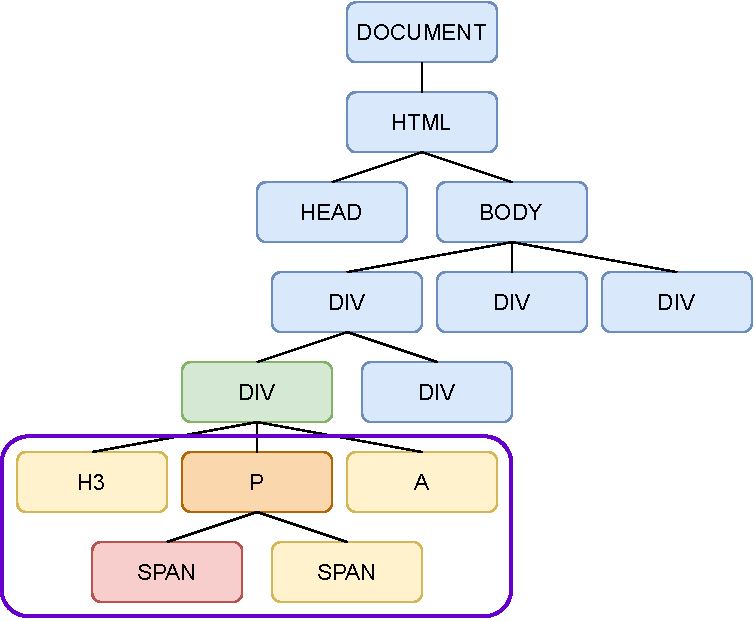
\includegraphics[width=0.9\textwidth]{obrazky-figures/dom.pdf}
	\caption{Vizuálna reprezentácia algoritmu používaného pri extrakcii}
	\label{domvisual}
\end{figure}

\newpage

\subsection{Príprava výsledkov}

V rámci generovania výsledkov prebieha aj ich finálna príprava pred zápisom. Vygenerované výsledky sú v rámci programu najskôr reprezentované len ako všeobecné prvky, ktorých dátový typ nie je určený a ich zaradenie je ekvivalentné. Následne prebehne odstránenie prípadných vzniknutých duplikátov na úrovni objektov. 

Príprava výsledkov pozostáva z určenia dátového typu a príslušnosti daného prvku. V prípade, že takéto určenie nie je možné, je prvok označený ako \textit{undefined}. Algoritmus analyzuje objekt na úrovni kľúčov a využíva špecifické pravidlá na zaradenie prvku k jeho príslušnej očakávanej reprezentácií. Ako prvé prebehne kontrola na výskyt prvku v zozname \textit{blacklist}. Ak sa kľúč v tomto zozname nachádza, nie je ďalej určovaný jeho dátový typ a je z objektu vyradený. 

V opačnom prípade prebehne kontrola na základe pravidiel definovaných vo vstupných súboroch. Tie sú reprezentované pomocou regulárnych výrazov. Jednotlivé prvky sa teda porovnávajú s regulárnymi výrazmi. V prípade, že prebehne zaradenie prvku splnením testu na regulárny výraz, je určený jeho dátový typ na základe príslušnosti regulárneho výrazu k definovanému dátovému typu. Následne je vytvorený nový objekt s prvkami, ktoré bolo možné zaradiť a tak im určiť príslušnosť. Zoznam všetkých takýchto objektov je potom naformátovaný do podoby JSON, a s \textit{UTF8} kódovaním uložený v rámci výstupnej lokácie. 

\bigskip

Po vygenerovaní výsledkov pre každý webový dokument v danej extrakčnej úlohe, sú zároveň vygenerované metadáta a extrakcia je ukončená. Ak extrakcia skončí úspešne, je o~tejto udalosti používateľ informovaný. Zároveň je zobrazený čas v milisekundách určujúci dĺžku extrakcie.

\chapter{Testovanie a vyhodnotenie výsledkov}
\label{testing}

Aplikačné testovanie a vyhodnotenie dosiahnutých výsledkov je veľmi dôležitou súčasťou tvorby každého projektu. Preto sa táto kapitola zameriava práve na zhodnotenie výsledkov, ktoré vyvinutá aplikácia dosiahla. 

Testovanie prebiehalo do určitej časti zároveň s vývojom aplikácie, avšak rozsiahlejšie testy boli uskutočnené až s vytvorením rôznych diverzifikovaných testovacích sád.

Testovanie pomocou týchto testovacích sád zároveň prebehlo na dvoch operačných systémoch, a to Windows 10 a Linux Manjaro. Pri testovaní a porovnávaní výsledkov medzi danými operačnými systémami nebola pozorovaná žiadna odchýlka alebo anomália. 

\section{Testovanie počas vývoja}

K testovaniu bolo pristupované od samotného začiatku vývoja a priebežné výsledky boli konzultované s vedúcim práce. Hlavnou úlohou tohto typu testovania bolo detegovanie chýb, anomálií a neočakávaných výstupov. Zároveň slúžilo na usmernenie vývoja a tvorbu nových funkcií. To sa z väčšej časti podarilo. K prvotnému návrhu pribudli nové funkcie a vylepšenia. Niektoré z nich sa stali základnou zložkou programu a jeho neoddeliteľnou súčasťou, zatiaľ čo iné ostali zapracované ako voliteľné. V prípade voliteľných sa jednalo zväčša o~funkcie a vlastnosti upresňujúce danú extrakčnú úlohu.

\section{Testovacie prostredie}

Ako už bolo spomenuté v úvode tejto kapitoly, testovacie prostredie z pohľadu operačného systému pozostávalo z nasledovných systémov:

\begin{itemize}
    \item Windows 10
    \item Linux Manjaro
\end{itemize}

\newpage

Čo sa webového prehliadača týka, použitá technológia Puppeteer nedokáže komunikovať s iným prehliadačom ako je Google Chrome\footnote{V čase vývoja a testovania aplikácie. Avšak podpora iných prehliadačov nieje v budúcnosti vylúčená.}. V jej základnej verzii dokonca prináša v~rámci inštalácie vlastný webový prehliadač, ktorým je práve prehliadač Chrome konkrétne vo~verzii Chromium 86.0.4240.0. Pri každej inštalácii Puppeteer nainštaluje najnovšiu verziu prehliadača, a preto sa mnou používaná verzia v budúcnosti nemusí s inštalovanou zhodovať. Zachovanie kompatibility by ale malo byť zabezpečené, keďže o vývoj obidvoch technológií sa stará spoločnosť Google.

Obmedzenie na prehliadač Chromium sa môže zdať ako limitujúci faktor, avšak level integrácie, ktorý vďaka tomu dokáže technológia Puppeteer dosiahnuť, prevyšuje všetky nedostatky.

\section{Spôsob testovania}
\label{sposobytestu}

Prvotné testovanie bolo uskutočňované manuálne. Po extrakcii údajov z webovej stránky boli tieto údaje manuálne skontrolované a overená integrita dát. 

V neskoršej fáze vývoja bol vyvinutý automatizačný skript pomocou programovacieho jazyka Python. Tento skript mal za úlohu porovnať očakávané údaje a údaje, ktoré aplikácia pri danej extrakčnej úlohe dokázala získať. Pri takomto porovnávaní bolo nutné zaviesť dve hlavné metriky \cite{precrecall}:

\begin{itemize}
    \item \textbf{Precision} a teda presnosť, ktorá má za úlohu odpovedať na otázku aká časť extrahovaných dát bola extrahovaná správne. Výsledná presnosť je vypočítaná nasledovným vzťahom:
    
    \begin{eqnarray}
    \label{preeq}
    Precision \quad = & {\displaystyle\frac{ROR}{ROR + ROI}}
    \end{eqnarray}
   
    Kde \textit{ROR} predstavuje počet všetkých extrahovaných objektov, ktoré sú pre nás relevantné a \textit{ROI} predstavuje počet irelevantných objektov. Týmto vzťahom vieme získať výslednú presnosť extrakcie dosiahnutú aplikáciou.
    
    \item \textbf{Recall}, ktorá odpovedá na otázku aká časť relevantných extrahovaných dát predstavuje očakávané dáta. Výsledná hodnota recall je preto daná vzťahom:
    
    \begin{eqnarray}
    \label{receq}
    Recall \quad = & {\displaystyle\frac{ROR}{EOR}}
    \end{eqnarray}
    
    Kde \textit{ROR} znova reprezentuje počet všetkých extrahovaných objektov, ktoré sú pre extrakciu relevantné a \textit{EOR} reprezentuje počet všetkých relevantných očakávaných objektov.
\end{itemize}

\bigskip

Pomocou týchto metrík bolo následne testovanie upresnené a výsledné hodnoty určili mieru presnosti extrakcie. Webové stránky sa môžu kedykoľvek zmeniť. Preto pre nutnosť zachovania integrity dát webovej stránky bolo dôležité webovú stránku stiahnuť na lokálny disk a následne ju z neho načítavať. Webovú stránku je ale nutné stiahnuť aj so všetkými závislosťami, a tak zachovať jej vzhľad a štruktúru. Stiahnutie webovej stránky konvenčnými nástrojmi alebo stiahnutie pomocou webového prehliadača nedokázalo dosiahnuť požadované výsledky. Za týmto účelom bol využitý nástroj \texttt{Save Page WE}\footnote{\url{https://chrome.google.com/webstore/detail/save-page-we/dhhpefjklgkmgeafimnjhojgjamoafof}}. Tento nástroj umožnil stiahnutie webovej stránky so všetkými závislosťami tak, že vzhľad a štruktúra zostali vo väčšine prípadoch zachované. Zároveň neboli pozorované žiadne výrazné anomálie a zmeny. Extrahovanie z live verzie stránky a z offline verzie bolo v konečnej fáze ekvivalentné. 

Testovanie si taktiež vyžiadalo vytvorenie spoľahlivej testovacej sady, ktorá by bola schopná úspešnosť aplikácie overiť vo viacerých prípadoch použitia. 

\section{Testovacia sada}
\label{dataset}

Vytvorenie spoľahlivej a dostatočne diverzifikovanej testovacej sady nie je jednoduchá úloha, a preto jej vytvorenie prebiehalo v spolupráci s autorom, ktorý rieši prácu na podobnú tému~\cite{mastera}. Táto skutočnosť bola riadne komunikovaná aj s vedúcim práce.

Finálna testovacia sada pozostávala zo 4 oblastí:

\begin{itemize}
    \item Futbalové výsledky a program zápasov
    \item Eshop www.tsbohemia.cz
    \item Eshopy
    \item Správy a novinky
\end{itemize}

Kde prvé dve oblasti boli pripravené mnou a posledné dve boli pripravené autorom druhej práce. Každá z týchto sád obsahuje 10 webových dokumentov. Všetky originálne URL adresy sú zároveň dostupné v rámci súboru \textit{INFO.md} v zložke \textit{dataset}.

\subsection{Štruktúra testovacej sady}

Základom každej testovacej sady je zložka s HTML súbormi, ktoré predstavujú jednotlivé webové dokumenty a ich očakávané extrahované hodnoty v druhej zložke. Očakávané hodnoty sú reprezentované JSON súbormi, kde každý nesie názov webového dokumentu, ktorého dáta predstavuje. 

Zároveň sú súčasťou každej testovacej sady súbory \textit{config.json} a \textit{data.json}, ktoré sú neoddeliteľnou súčasťou aplikácie a bližšie špecifikujú extrakčnú úlohu pri danej testovacej sade. Extrahované dáta sú následne uložené do zložky \textit{output}.

Jedna testovacia sada reprezentovaná práve jednou oblasťou má teda nasledovnú štruktúru, ktorá je zároveň kľúčová pre testovací skript a musí byť dodržaná:

\bigskip

\dirtree{%
.1 Názov\_oblasti.
.2 domains/\DTcomment{Obsahuje HTML súbory s webovými dokumentami}.
.2 expected/\DTcomment{Obsahuje JSON súbory s očakávanými dátami}.
.2 output/\DTcomment{Obsahuje JSON súbory s vygenerovanými dátami}.
.2 config.json\DTcomment{Predstavuje konfiguračný súbor aplikácie}.
.2 data.json\DTcomment{Predstavuje vstupný súbor s používateľskými dátami}.
}

\bigskip

Pri kontrole výsledkov využíva testovací skript zložky expected a output, kde počet súborov v týchto zložkách musí byť zhodný.

Po spustení aplikácie za účelom testu takejto sady, sú zároveň vygenerované metadáta do koreňového adresára tejto sady, teda vo výsledku sa budú nachádzať v rovnakom adresári ako config.json a data.json.


\section{Testovací skript}

Za účelom rýchlejšej a spoľahlivejšej kontroly bol vyvinutý testovací skript v programovacom jazyku Python. Nesie názov \textit{ftest.py} a porovnáva vzájomne dva JSON súbory z jednej testovacej oblasti: Jeden zo zložky expected a druhý zo zložky output. Pri porovnávaní berie v úvahu metriky spomenuté v sekcii \ref{sposobytestu}.

Skript berie ako parameter názov testovacej oblasti, čo je zároveň názov koreňového adresáru jednej testovacej sady. Po kontrole štruktúry adresára sú načítané jednotlivé JSON súbory a skript začína s porovnávaním.

V prípade, že dva porovnávané súbory obsahujú rovnaký počet objektov, prebieha porovnávanie na úrovni kľúčov, pretože sa dá postupovať jednoznačným spôsobom a porovnávať jednotlivé kľúče objektov, čo vedie k presnejšiemu vyhodnoteniu. 

Ak ale dva súbory neobsahujú rovnaký počet objektov, je veľmi zložité priradiť jednotlivé kľúče k jednotlivým objektom. V takom prípade skript prechádza k menej presnému porovnávaniu na úrovni objektov. Vtedy je pre úspešnosť porovnania potrebná reprezentácia objektu 1:1, teda extrahovaný objekt sa musí nachádzať v súbore s očakávanými dátami.

Pri každom irelevantnom kľúči alebo objekte je pripočítaná hodnota k počtu irelevantných prvkov. Na záver, potom ako sú obidva súbory skontrolované, skript vygeneruje výsledné hodnoty precision a recall. Zároveň si skript drží internú pamäť týchto čiastkových výsledkov a po skončení testovania jednej testovacej sady, vygeneruje priemernú hodnotu precision a recall.

Pri spustení skriptu s parametrom \textit{-o} sú zároveň tieto priemerné hodnoty zapísané do dočasného súboru overall. Po otestovaní viacerých testovacích sád je následne možné spustiť skript \textit{overall.py}, ktorý vypočíta priemernú váženú hodnotu precision a priemernú váženú hodnotu recall.

\bigskip

Skript po spustení otestuje určenú testovaciu sadu a vygeneruje výsledky. Tie sa skladajú z nasledovných údajov:

\begin{itemize}
    \item \textbf{Status}: určuje status kontroly daného webového dokumentu,
    \item \textbf{Precision}: hodnota precision pre daný webový dokument,
    \item \textbf{Recall}: hodnota recall pre daný webový dokument,
    \item \textbf{Domain}: názov súboru s očakávanými výsledkami (nesie názov webového dokumentu).
\end{itemize}

\bigskip

Na záver sú vypísané priemerné výsledky pre testovanú sadu.

\bigskip

Vytvorenie tohto testovacieho skriptu bolo zároveň kľúčové pre celkové zhodnotenie výsledkov. Pri takom množstve súborov, aké sa v testovacej sade nachádza, by manuálna kontrola a vyhodnotenie prebiehalo len veľmi ťažko.

\newpage

\section{Vyhodnotenie testovacích sád}

Pri vyhodnocovaní výsledkov boli využité metriky spomínané v sekcii \ref{sposobytestu} a testovacie sady zo sekcie \ref{dataset}. Testovacia sada \uv{Správy a novinky} bola pri testovaní z dôvodu lepšieho určenia požiadaviek a regulárnych výrazov rozdelená na dve. Celkové vyhodnotenie výsledkov prináša možnosť overiť kvalitu výslednej aplikácie, a preto je správne vyhodnotenie výsledkov veľmi dôležité. 

Nejedná sa totiž len o jednoduché vyobrazenie výsledných dát a porovnanie ich reprezentácie s očakávanými údajmi. Táto metrika nám napovie, kde aplikácia dominuje, a kde zlyháva. Stále je však potrebné zvážiť aj koreláciu a kauzalitu týchto výsledkov. 

V úvode tejto kapitoly bola uvedená skutočnosť, že na výsledné hodnoty nemá zmena operačného systému významný vplyv. Pri vyhodnocovaní bol teda použitý operačný systém Windows 10 vo verzii 20H2.

Webové prehliadače vyžadujú pre načítanie webového dokumentu jeho absolútnu cestu. Pre zaručenie prenositeľnosti testovacích sád boli však v  týchto sadách uvádzané cesty relatívne. Pre správne spustenie testov a zaručenie nahradenia relatívnych ciest, je preto vyžadované spustenie aplikácie s parametrom \texttt{-{}-dataset}. Použitie relatívnej cesty predpokladá umiestnenie testovacích sád v zložke \texttt{/tests/dataset/}, z pohľadu koreňového adresára aplikácie.

Všetky testy sú zároveň spustiteľné pomocou priloženého súboru \textit{Makefile}. Jeho možnosti a dostupné parametre sú popísané v \textit{README.md} súbore priloženom v koreňovom adresári aplikácie alebo v rámci manuálu dostupného v prílohe \ref{manual}.

\bigskip

Pri vyhodnocovaní výsledkov boli taktiež zohľadnené údaje, ktoré sú generované v rámci extrakcie. Tieto údaje neboli generované výsledným testovacím skriptom a sú viazané na aktivitu aplikácie.

Všetky časové údaje pri výsledkoch testovacích sád predstavujú priemernú hodnotu z 5 pokusov, ich hodnota je zaokrúhlená na celé milisekundy a ďalej:

\begin{itemize}
    \item \textbf{OC}: počet extrahovaných objektov,
    \item \textbf{aTime}: čas potrebný na detekciu a analýzu primárneho prvku,
    \item \textbf{eTime}: čas potrebný na určenie príslušnosti a finálnu extrakciu údajov,
    \item \textbf{lTime}: čas potrebný na načítanie webového dokumentu.
\end{itemize}

\bigskip

Tieto údaje budú používané v rámci tabuliek zobrazujúcich výsledky pre jednotlivé domény v testovacích sadách. Je treba samozrejme brať v úvahu povahu offline dokumentu z pohľadu doby načítavania. Pri offline dokumentoch bude táto doba jednoznačne nižšia ako pri extrakcii z online dokumentov. 

Po vyhodnotení jednotlivých testovacích sád bude zároveň vyhodnotené testovanie ako také. Priemerné hodnoty zo všetkých 40 dokumentov vytvoria dobrú predstavu o funkčnosti a použiteľnosti aplikácie.

\newpage

\subsubsection{Futbalové výsledky a program zápasov}
\label{football}

Testovacia sada zameraná na futbalové výsledky je zameraná na webové stránky zobrazujúce informácie o futbalových zápasoch. Táto sada bola zvolená pre fakt, že takéto stránky sa síce na prvý pohľad zdajú podobné, avšak nie vždy je to pravda. 

Niektoré obsahujú informácií viac, niektoré menej. Niektoré obsahujú veľké množstvo irelevantných dát. Tie je však nutné odfiltrovať. Iné naopak obsahujú len očakávané dáta.

\bigskip

Ako cielené dáta boli určené čas, názov domáceho týmu, skóre a názov hosťujúceho týmu. Za primárny prvok bol zvolený časový údaj. Štruktúra vstupných dát preto vyzerá nasledovne:

\bigskip

\begin{lstlisting}
"structure":{
        "time": "time",
        "team1": "string",
        "score": "score",
        "team2": "string"
}
\end{lstlisting}

\bigskip

Z vygenerovaných údajov teda vieme vytvoriť nasledovnú tabuľku:

\begin{table}[hbt]
\caption{Výsledné hodnoty testovacej sady futbalové výsledky}
\centering
\begin{tabular}{|l|l|l|l|l|l|l|}
\hline
\textbf{Doména}          & \textbf{Precision} & \textbf{Recall}  & \textbf{OC}  & \textbf{aTime} & \textbf{eTime} & \textbf{lTime}  \\ \hline
365scores.com   & 100,0\%   & 100,0\% & 18  & 114ms & 5ms   & 995ms  \\ \hline
777score.com    & 100,0\%   & 100,0\% & 154 & 92ms  & 15ms  & 1158ms \\ \hline
LiveScore.com   & 100,0\%   & 99,07\% & 81  & 90ms  & 5ms   & 852ms  \\ \hline
SkySports.com   & 100,0\%   & 100,0\% & 200 & 114ms & 22ms  & 849ms  \\ \hline
Soccerstand.com & 100,0\%   & 98,64\% & 110 & 67ms  & 11ms  & 1192ms \\ \hline
bbc.com         & 100,0\%   & 100,0\% & 47  & 66ms  & 3ms   & 759ms  \\ \hline
flashscore.com  & 100,0\%   & 98,66\% & 112 & 76ms  & 8ms   & 1411ms \\ \hline
flashscore.sk   & 100,0\%   & 66,95\% & 79  & 154ms & 7ms   & 1502ms \\ \hline
scoreboard.com  & 92,84\%   & 47,73\% & 110 & 103ms & 10ms  & 1265ms \\ \hline
soccer24.com    & 86,14\%   & 53,93\% & 80  & 292ms & 10ms  & 1516ms \\ \hline
\end{tabular}
\end{table}

Vykonanie extrakcie na týchto 10 webových dokumentov priemerne trvalo 13627ms, čo nám dáva hodnotu 1362,7ms na jeden dokument. 

Z tejto hodnoty pripadá priemerne 116,8ms na aTime (8,6\%), 9,6ms na eTime (0,7\%) a~1149,9ms na lTime (84,39\%). Zostávajúci čas (6,31\%) pripadal na réžiu aplikácie. Priemerná úspešnosť predstavovala hodnotu 97,9\% a priemerná hodnota recall hodnotu 86,5\%. 

\bigskip

Z následnej analýzy výsledkov a detailnej analýzy webových dokumentov sa podarilo zistiť, že strata na hodnotách recall je daná princípom fungovania aplikácie.

Aplikácia združuje elementy na základe ich atribútu triedy. Avšak, v niektorých prípadoch, ak sa časový údaj športového záznamu zmenil na \uv{Finished} alebo \uv{Canceled},  nastala zároveň zmena atribútu triedy. Aplikácia tak tieto záznamy nezaradila do výsledkov, a preto boli stratené.

\newpage

\subsubsection{Eshop www.tsbohemia.cz}

Testovacia sada bola zameraná na extrahovanie údajov z rôznych kategórií produktov eshopu tsbohemia. Sada predstavuje webové dokumenty z jednej domény, avšak aj v rámci jednej domény môžu vzniknúť anomálie medzi jednotlivými dokumentami.

Anomálie môžu predstavovať odlišné zaradenie produktov, rôzne reprezentácie ceny a~absenciu niektorých vyhľadávaných prvkov(napríklad absencia zľavy niektorých objektov). Zároveň však tento fakt predstavuje výhodu, pretože sa vstupné pravidlá dajú vzniknutým anomáliám prispôsobiť lepšie, ako pri extrakcii z viacerích domén.

\bigskip

Ako cielené dáta boli určené nadpis produktu, cena, popis produktu a zľava. Za primárny prvok bol zvolený údaj o cene. Štruktúra vstupných dát preto vyzerá nasledovne:

\bigskip

\begin{lstlisting}
"structure":{
        "title": "string_title",
        "price": "price",
        "description": "string_desc",
        "discount": "discount"
}
\end{lstlisting}

\bigskip

Z vygenerovaných údajov teda vieme vytvoriť nasledovnú tabuľku:

\begin{table}[hbt]
\caption{Výsledné hodnoty testovacej sady tsbohemia}
\centering
\begin{tabular}{|l|l|l|l|l|l|l|}
\hline
\textbf{Dokument}          & \textbf{Precision} & \textbf{Recall}  & \textbf{OC}  & \textbf{aTime} & \textbf{eTime} & \textbf{lTime}  \\ \hline
brusky.html     & 100,0\%   & 100,0\% & 24 & 52ms  & 13ms  & 1014ms \\ \hline
chladice.html   & 100,0\%   & 100,0\% & 24 & 60ms  & 10ms  & 1045ms \\ \hline
chladnicky.html & 100,0\%   & 100,0\% & 24 & 57ms  & 9ms   & 895ms  \\ \hline
disky.html      & 100,0\%   & 100,0\% & 24 & 48ms  & 9ms   & 905ms  \\ \hline
kolobezky.html  & 100,0\%   & 100,0\% & 24 & 51ms  & 9ms   & 834ms  \\ \hline
mobo.html       & 100,0\%   & 100,0\% & 24 & 53ms  & 7ms   & 1010ms \\ \hline
monitory.html   & 100,0\%   & 100,0\% & 24 & 68ms  & 8ms   & 924ms  \\ \hline
proc.html       & 100,0\%   & 100,0\% & 24 & 54ms  & 10ms  & 980ms  \\ \hline
servery.html    & 100,0\%   & 100,0\% & 24 & 61ms  & 9ms   & 959ms  \\ \hline
skenery.html    & 100,0\%   & 100,0\% & 24 & 43ms  & 10ms  & 797ms  \\ \hline
\end{tabular}
\end{table}

Vykonanie extrakcie na týchto 10 webových dokumentov priemerne trvalo 10876ms, čo nám dáva hodnotu 1087,6ms na jeden dokument. 

Z tejto hodnoty pripadá priemerne 54,7ms na aTime (5,02\%), 9,4ms na eTime (0,86\%) a~936,3ms na lTime (86,08\%). Zostávajúci čas (8,04\%) pripadal na réžiu aplikácie. Priemerná úspešnosť predstavovala hodnotu 100,0\% a hodnota recall hodnotu 100,0\%. 

\bigskip

Celková úspešnosť 100\% je daná faktom, že pri extrahovaní dát z rovnakej domény je zadefinovanie jednoznačných vstupných pravidiel jednoduchšie. Pri rôznych doménach sa mení nielen štruktúra kódu, ale aj štruktúra dát. Ak extrakcia prebieha v rámci jednej domény, dá sa predpokladať, že medzi jednotlivými dokumentami budú existovať vzťahy a~podobnosti. Tie môžme následne využiť pri tvorbe definícií pravidiel.

\newpage

\subsubsection{Eshopy}

Testovacia sada v tomto prípade obsahovala eshopy v podobe rôznych domén. V testovacej sade sa nachádzajú najznámejšie eshopy z Českej republiky, ale aj menej známe a menšie eshopy na vytvorenie diverzity.

Eshopy zobrazujú odlišné produkty, kategórie a odlišný počet objektov. Každý eshop má zároveň vlastnú reprezentáciu zľavy, zobrazenia ceny a v neposlednom rade popisu produktov. V tomto zmysle sa jedná o veľmi diverzifikovanú testovaciu sadu.

\bigskip

Ako cielené dáta boli určené názov produktu, cena, popis produktu a zľava. Za primárny prvok bol zvolený údaj o cene. Štruktúra vstupných dát preto vyzerá nasledovne:

\bigskip

\begin{lstlisting}
"structure": {
        "name": "string_title",
        "price": "price",
        "description": "string_desc",
        "sale": "discount"
}
\end{lstlisting}

\bigskip

Z vygenerovaných údajov teda vieme vytvoriť nasledovnú tabuľku:

\begin{table}[hbt]
\caption{Výsledné hodnoty testovacej sady eshopy}
\centering
\begin{tabular}{|l|l|l|l|l|l|l|}
\hline
\textbf{Doména}          & \textbf{Precision} & \textbf{Recall}  & \textbf{OC}  & \textbf{aTime} & \textbf{eTime} & \textbf{lTime}  \\ \hline
alza.cz                 & 5,56\%    & 1,16\%  & 6  & 186ms & 7ms   & 1014ms \\ \hline
czc.cz                  & 66,67\%   & 63,53\% & 27 & 93ms  & 20ms  & 809ms  \\ \hline
insportline.cz          & 72,88\%   & 57,59\% & 59 & 86ms  & 25ms  & 1211ms \\ \hline
papirnictvieshop.cz     & 100,0\%   & 100,0\% & 20 & 123ms & 23ms  & 741ms  \\ \hline
smarty.cz               & 40,28\%   & 32,95\% & 24 & 86ms  & 30ms  & 875ms  \\ \hline
sparkys.cz              & 75,0\%    & 75,0\%  & 12 & 78ms  & 7ms   & 1061ms \\ \hline
stavebninystastny.cz    & 100,0\%   & 100,0\% & 10 & 67ms  & 21ms  & 758ms  \\ \hline
tsbohemia.cz.html       & 87,18\%   & 87,18\% & 24 & 64ms  & 13ms  & 849ms  \\ \hline
zahradkarske-potreby.cz & 66,67\%   & 66,67\% & 15 & 73ms  & 9ms   & 971ms  \\ \hline
zahradnictvi-spomysl.cz & 100,0\%   & 100,0\% & 38 & 149ms & 23ms  & 905ms  \\ \hline
\end{tabular}
\end{table}

Vykonanie extrakcie na týchto 10 webových dokumentov priemerne trvalo 11228ms, čo nám dáva hodnotu 1122,8ms na jeden dokument. 

Z tejto hodnoty pripadá priemerne 100,5ms na aTime (8,95\%), 17,8ms na eTime (1,59\%) a 919,4ms na lTime (81,88\%). Zostávajúci čas (7,58\%) pripadal na réžiu aplikácie. Výsledná priemerná úspešnosť predstavovala hodnotu 71,42\% a priemerná hodnota recall hodnotu 68,41\%. 

\bigskip

Po analyzovaní webových dokumentov bolo možné vyvodiť záver a príčiny výsledkov. Znížená úspešnosť bola zapríčinená viacerými faktormi. Dva hlavné faktory boli opakovaný výskyt cenovej hodnoty v jednom objekte a zložitá štruktúra webového dokumentu. Ak jedna cena v rámci objektu predstavovala cenu bez DPH alebo pred zľavou a v rámci DOM sa nachádzala na bližšom indexe, bola určená za výslednú. V prípade zložitosti dokumentu, ak bol objekt rozdelený na vyššom indexe rodičovského prvku z pohľadu DOM, prichádzalo k nesprávnemu zaradeniu detských elementov.

\newpage

\subsubsection{Správy a novinky}
\label{spravy}

V tomto prípade sa jedná o sadu zameranú na správy a novinky. Narozdiel od iných sád je v tejto väčšie množstvo textových elementov, medzi ktorými treba rozlišovať. Zároveň sa líšia v reprezentácií časového údaju. Niektoré reprezentujú čas ako dátum, iné v podobe času uplynulého od zverejnenia. 

Testovacia sada bola zároveň z dôvodu lepšieho špecifikovania vstupných údajov rozdelená na dve.

\bigskip

Za cielené dáta boli určené autor, nadpis článku, časový údaj a popis článku. Za primárny prvok bol zvolený časový údaj. Štruktúra vstupných dát preto vyzerá nasledovne:

\bigskip

\begin{lstlisting}
"structure":{
        "author": "string_author",
        "title": "string_title",
        "timestamp": "timestamp",
        "synopsis": "string_synopsis"
}
\end{lstlisting}

\bigskip

Z prvej časti testovacej sady vieme vytvoriť nasledovnú tabuľku:

\begin{table}[hbt]
\caption{Výsledné hodnoty testovacej sady Správy a novinky (prvá časť)}
\centering
\begin{tabular}{|l|l|l|l|l|l|l|}
\hline
\textbf{Doména}          & \textbf{Precision} & \textbf{Recall}  & \textbf{OC}  & \textbf{aTime} & \textbf{eTime} & \textbf{lTime}  \\ \hline
artnews.com             & 72,5\%    & 72,5\%  & 10 & 127ms & 7ms   & 1993ms \\ \hline
ceskymac.cz             & 100,0\%   & 100,0\% & 20 & 47ms  & 13ms  & 1013ms \\ \hline
cyclingnews.com         & 96,67\%   & 72,5\%  & 20 & 88ms  & 7ms   & 781ms  \\ \hline
pcgamer.com             & 93,33\%   & 70,0\%  & 20 & 84ms  & 7ms   & 778ms  \\ \hline
podnikatel.cz           & 16,67\%   & 3,25\%  & 8  & 47ms  & 6ms   & 923ms  \\ \hline
rockpapershotgun.com    & 69,0\%    & 69,0\%  & 25 & 70ms  & 7ms   & 1034ms \\ \hline
smartmania.cz           & 100,0\%   & 100,0\% & 22 & 37ms  & 12ms  & 896ms  \\ \hline
\end{tabular}
\end{table}

Vykonanie extrakcie na 7 webových dokumentoch priemerne trvalo 8846,4ms, čo nám dáva hodnotu 1263,77ms na jeden dokument. 

Z tejto hodnoty pripadá priemerne 70,43ms na aTime (5,58\%), 8,43ms na eTime (0,67\%) a 1059,71ms na lTime (83,85\%). Zostávajúci čas (9,9\%) pripadal na réžiu aplikácie. Výsledná priemerná úspešnosť predstavovala hodnotu 78,31\% a priemerná hodnota recall hodnotu 69,61\%. 

\bigskip

Analýza jednotlivých dokumentov ukázala, že znížené hodnoty precision a recall v niektorých prípadoch korelujú s udalosťou, kde dochádza ku spojeniu jednotlivých prvkov do jedného. Stáva sa tak hlavne pri dvojici \uv{author} a \uv{timestamp}, kde sú tieto dve hodnoty často reprezentované v rámci jedného extrahovaného DOM elementu. Aplikácia následne túto hodnotu určí ako jednu z vyhovujúcich na základe toho, ktorý regulárny výraz splní podmienku daného prvku. Toto je spôsobené väčším množstvom textových elementov. Zadefinovanie jednoznačného regulárneho výrazu pre každý z nich tak, aby sa neprekrývali, je preto zložitejšie.

\newpage

Druhá časť testovacej sady obsahuje 3 webové dokumenty a z výsledkov vieme vytvoriť nasledovnú tabuľku:

\begin{table}[hbt]
\caption{Výsledné hodnoty testovacej sady Správy a novinky (druhá časť)}
\centering
\begin{tabular}{|l|l|l|l|l|l|l|}
\hline
\textbf{Doména}          & \textbf{Precision} & \textbf{Recall}  & \textbf{OC}  & \textbf{aTime} & \textbf{eTime} & \textbf{lTime}  \\ \hline
google.com              & 66,67\%   & 50,0\%  & 10 & 77ms  & 10ms  & 1016ms \\ \hline
mndaily.com             & 47,62\%   & 75,0\%  & 18 & 44ms  & 14ms  & 890ms  \\ \hline
techcrunch.com          & 64,86\%   & 50,0\%  & 24 & 63ms  & 11ms  & 1061ms \\ \hline
\end{tabular}
\end{table}

Vykonanie extrakcie na 3 webových dokumentoch priemerne trvalo 	4038,2ms, čo nám dáva hodnotu 1346,07ms na jeden dokument. 

Z tejto hodnoty pripadá priemerne 61,34ms na aTime (4,56\%), 11,67ms na eTime (0,87\%) a 989ms na lTime (73,47\%). Zostávajúci čas (21,1\%) pripadal na réžiu aplikácie. Priemerná úspešnosť predstavovala hodnotu 59,72\% a priemerná hodnota recall hodnotu 58,33\%. 

\bigskip

Z analýzy vyplýva rovnaký záver ako pri prvej časti tejto testovacej sady. 

\bigskip

Priemerná vážená úspešnosť sady Správy a novinky je teda 72,73\% precision a 66,23\% hodnota recall.

\section{Vyhodnotenie výsledkov}

Po vyhodnotení všetkých testovacích sád vieme vytvoriť obraz o celkovej úspešnosti aplikácie. Tá dosiahla z pomedzi všetkých výsledkov nasledovné priemerné vážené hodnoty:

\begin{itemize}
    \item \textbf{Precision:} 85,51\%
    \item \textbf{Recall:} 80,28\%
\end{itemize}

Výsledné časové údaje ukázali, že priemerný časový úsek na spracovanie jedného dokumentu je 1215,38ms. Toto číslo však platí pre súbory offline testovacej sady a v reálnom svete pri extrahovaní z online webových dokumentov bude extrahovanie pomalšie. To ako veľmi pomalšie už závisí od štruktúry webového dokumentu, obsahu, serveru a mnohých ďalších aspektov.

Z časových údajov nevyplynula žiadna významná korelácia, avšak jednotlivé hodnoty \texttt{precision} a \texttt{recall} vykazujú na základe Pearsonovho korelačného koeficientu silnú pozitívnu korelačnú závislosť \cite{statistics}. Túto vieme vypočítať vzorcom \ref{correlation}:

\begin{eqnarray}
\label{correlation}
    r = \frac{{}\sum_{i=1}^{n} (x_i - \overline{x})(y_i - \overline{y})}
{\sqrt{\sum_{i=1}^{n} (x_i - \overline{x})^2(y_i - \overline{y})^2}}
    \end{eqnarray}

Kde $x_i$ reprezentuje hodnoty \textit{x} vo vzorke, $\overline{x}$ reprezentuje priemernú hodnotu \textit{x}, $y_i$ reprezentuje hodnoty \textit{y} vo vzorke a $\overline{y}$ reprezentuje priemernú hodnotu \textit{y}. Za hodnoty \textit{x} boli dosadené hodnoty precision, a za hodnoty \textit{y} boli dosadené hodnoty recall. Výsledná hodnota \textit{r}, ktorá reprezentuje Pearsonov korelačný koeficient, dosahuje čísla 0,8877. To indikuje, že vysoké hodnoty precision sú sprevádzané vysokými hodnotami recall a nízke hodnoty s~nízkymi. 

Z tohto faktu vieme ďalej vytvoriť predpoklad, že zlepšenie presnosti povedie k získaniu viacerých relevantných výsledkov. Zlepšenie v tomto zmysle nemusí byť viazané na logiku aplikácie, ale môže byť viazané aj na presnosť definovaného regulárneho výrazu. Ak bude definovaný regulárny výraz príliš všeobecný, bude presnosť nižšia. To sme mohli pozorovať aj pri testovacej sade \uv{Správy a novinky} \ref{spravy} z dôvodu väčšieho počtu textových elementov.

\section{Paralelizácia načítania webstránok}

Z výsledkov vyplýva aj fakt, že najväčší časový úsek zaberá jednotlivé načítavanie webových dokumentov. Načítavanie dokumentov zaberalo približne 81,93\% celkového času potrebného na extrakciu. Nad rámec zadania bakalárskej práce som implementoval paralelizáciu tohto načítavania. Paralelizácia spočíva v súčasnom načítavaní poskytnutých webových stránok, kde v prípade veľkého množstva stránok je možné načítavanie rozdeliť do skupín tak, aby bolo zaťaženie rozložené.

Výsledky sú v rámci testovacích sád jednoznačné. Pre porovnanie uvediem nové výsledky testovacej sady \uv{Futbalové výsledky a program zápasov} vyhodnotenej aj v sekcii \ref{football}:

\begin{table}[hbt]
\caption{Výsledné hodnoty testovacej sady futbalové výsledky s aktívnou paralelizáciou}
\centering
\begin{tabular}{|l|l|l|l|l|l|l|}
\hline
\textbf{Doména}          & \textbf{Precision} & \textbf{Recall}  & \textbf{OC}  & \textbf{aTime} & \textbf{eTime} & \textbf{lTime}  \\ \hline
365scores.com   & 100,0\%   & 100,0\% & 18  & 156ms & 7ms   & 1589ms  \\ \hline
777score.com    & 100,0\%   & 100,0\% & 154 & 163ms  & 19ms  & 1722ms \\ \hline
LiveScore.com   & 100,0\%   & 99,07\% & 81  & 138ms  & 8ms   & 2045ms  \\ \hline
SkySports.com   & 100,0\%   & 100,0\% & 200 & 175ms & 23ms  & 3630ms  \\ \hline
Soccerstand.com & 100,0\%   & 98,64\% & 110 & 92ms  & 11ms  & 4637ms \\ \hline
bbc.com         & 100,0\%   & 100,0\% & 47  &  138ms  & 8ms  & 2045ms \\ \hline
flashscore.com  & 100,0\%   & 98,66\% & 112 & 230ms  & 25ms   & 2061ms \\ \hline
flashscore.sk   & 100,0\%   & 66,95\% & 79  & 326ms & 23ms   & 3032ms \\ \hline
scoreboard.com  & 92,84\%   & 47,73\% & 110 & 194ms & 16ms  & 3610ms \\ \hline
soccer24.com    & 86,14\%   & 53,93\% & 80  & 491ms & 14ms  & 3115ms \\ \hline
\end{tabular}
\end{table}

Z uvedených výsledkov je zrejmé, že čas potrebný na vykonanie jednotlivých častí extrakcie sa zvýšil. Priemerný čas analýzy a detekcie stúpol na hodnotu 210,4ms, čo predstavuje nárast o 80,14\% a čas potrebný na načítanie webovej stránky stúpol na hodnotu 2748,6ms, teda nárast o 139\%. Keďže sa ale jednalo o paralelné načítavanie, celkový čas potrebný na extrakciu klesol na priemernú hodnotu 8763,2ms. To predstavuje 35,69\% zníženie časových nárokov na extrakciu. Výsledné hodnoty týkajúce sa hodnoty precision a hodnoty recall však zostali zachované.

Paralelizmus je ale značne náročnejší čo sa týka požiadaviek na hardware. Najlepší výsledok, čo sa rýchlosti týka, bol prvý, kedy aplikácia dokázala danú úlohu vykonať za 6375ms. To by predstavovalo viac ako 53\% ušetreného času. Práve kvôli náročnosti, zaťaženiu a~zahriatiu hardware neskôr výsledky klesali na úroveň 9000-1000ms. Dá sa ale predpokladať, že pri dostatočne výkonnom hardware by paralelizácia mohla byť užitočná a~výsledky podávané v konštantnej časovej rovine.

Pri extrakcii z online zdrojov môžu vzniknúť ďalšie problémy týkajúce sa veľkého zaťaženia nielen PC, ale aj sieťového pripojenia. Dostatočne výkonný hardware by si ale s~takým zaťažením mal vedieť poradiť. Túto hypotézu však v súčasnom stave nemám ako overiť, a~preto možnosť paralelizmu nebola do výslednej aplikácie zaradená.


\chapter{Záver}

Výsledkom tejto bakalárskej práce je aplikácia určená na inteligentnú extrakciu dát z webových dokumentov. Extrakcia prebieha na základe dopredu definovaných pravidiel zložených z regulárnych výrazov a dátových typov. Hlavným cieľom bolo vytvoriť spôsob extrakcie tak, aby nezáležalo na štruktúre kódu, na ktorom je webový dokument postavený, ale na obsahu dokumentu. Tento cieľ sa podarilo splniť a vytvoriť tak aplikáciu, ktorá dokáže uľahčiť extrakciu pre bežných používateľov. Zároveň túto extrakciu značne automatizuje a~výsledky dosahuje v rozumných časových úsekoch.

Použitie a inštalácia aplikácie zostali napriek rôznym dostupným možnostiam jednoduché. Aplikácia podporuje radu parametrov upresňujúcich chovanie a vnútornú logiku pri rozhodovaní o zaradení výsledkov. Tieto parametre majú za úlohu špecifikovať danú extrakčnú úlohu. Aplikácia by aj bez zadania dodatočných parametrov mala spoľahlivo extrahovať požadované údaje.

Táto technická správa najskôr rozoberá aktuálne prístupy k problematike a popisuje dostupné technológie. Práve tieto rozbory a technológie udávali smerovanie nasledujúcich návrhov a implementačných detailov. 

Implementácia bola rozdelená do viacerých logických častí. Najskôr bola navrhnutá logika a následne bola táto logika rozvedená na zabezpečenie požadovaných výsledkov. Aplikácia bola ďalej rozšírená o funkcie, ktoré pomohli docieliť požadovanú kvalitu výsledkov.

Z testovania aplikácie vyplýva, že priemerná rýchlosť extrakcie sa pohybuje na úrovni 1215 milisekúnd, hodnota udávajúca priemernú presnosť je 85,61\% a priemerná hodnota recall 80,28\%. 

Aplikácia využíva moderné technológie ako napríklad Node.js, Puppeteer a Chromium. Vďaka technológii Node.js a jej modernému spôsobu spracovania modulov je navyše inštalácia závislostí jednoduchá a rýchla. Najdôležitejšou technológiou pre výslednú aplikáciu je práve Puppeteer. Táto technológia má podľa mňa veľký potenciál. Stretol som sa s ňou v~tejto práci prvýkrát, ale rýchlo som si osvojil jej vlastnosti a funkcie. Kvôli jej integrácii a funkcionalitám, ktoré ponúka dúfam, že v budúcnosti bude pokračovať jej vývoj a budem môcť pracovať na podobných projektoch alebo rozvíjať aktuálnu prácu.

Výsledná aplikácia dosahuje výsledky rýchlo a relatívne kvalitne, avšak vždy je miesto na zlepšenie. To by mohlo pozostávať z vytvárania vzťahov medzi rôznymi webovými dokumentami a extrahovanými údajmi alebo by aplikácia mohla vytvárať pri analýze webového dokumentu pomocné relačné vzťahy.
